
%%% Local Variables:
%%% mode: latex
%%% TeX-master: t
%%% End:



\chapter{弹性波波动方程反射FWI走时反演}

尽管常规FWI在长偏移距,宽方位数据中有着令人满意的效果,但是在这种观测系统下,
FWI主要利用了长偏移距透射波以及临界反射波所携带的信息来更新速度模型的
中长尺度波长的分量。但是中深部区域,FWI往往只能更新来自反射数据的高波数成分,中低尺度波数很难从透射数据中获得。
传统反射层析流程大量依赖人工拾取,使得速度建模极为耗时,且在弹性介质中,$V_s$模型难以获取,使得建立一种有效可靠的弹性介质建模方法迫在眉睫。

目前研究的热点就是想通过反射层析类似的思路,采用反射波波路径来更新中深部的速度模型。弹性波中,不同的速度更新需要找到相应的反射波路,也即
$V_p$与$V_s$的更新需要分别对应PP波与PS波波路径(假设P波震源)。这样就需要将波场中的P或S数据分量进行分离,使得在反演时能利用不同的数据分量,从而
降低非线性程度。但尽管如此,RWI中的强非线性问题仍然存在,尤其是在使用波形匹配的目标函数时。我们使用与速度更具有线性关系的走时信息
作为目标函数,而走时信息则采用Dynamic image warping获取。由于PP与PS走分别包含在在P波与S波地震记录中,因此还需要采用地面数据分离的方式
分解出P或S波数据,才能保证准确获取PP和PS波走时信息。本章中采用E-WERTI的方式,通过两步法的策略建立$V_p$与$V_s$的背景模型。

\section{引言}
弹性波全波形反演可以提供高精度的地下模型参数估计,但是也同样受困于多参数反演中的强烈
非线性程度以及声波情况下的周波跳跃问题\cite[]{sears:2008,brossier2009}。
利用反射波信息可以更好的照明深部,人们希望能利用反射波来更新中深部的背景速度模型。
WEMVA类方法通过引入扩展成像条件,最小化扩展道集上非零偏移距的能量来实现更新,如Sava and
Fomel(2006)\cite{SavaEtAl2006}; Yang and Sava(2011)\cite{YangEtAl2011}; Almomin and
Biondi(2012)\cite{Almomin2012}; Sun and Symes(2012)\cite{SunEtAl2012}。但WEMVA
受困于昂贵的计算代价,尤其实在三维问题中。
针对反射走时,Luo et
al(2016)\cite{Luo2016}用时间轴方向的扩展成像与Rytov近似结合,导出了全走时反演(FTI)获得了不错的反演效果,但其实质上也是一种成像域的反演方法。

在数据域同样可以实现反射波对模型的深部更新。受MBTT方法的启发,Xu et al (2012)\cite{xu:2012}
提出了反射波波形反演方法(RWI)。RWI先采用RTM或LSRTM的方式获取反射率,
然后用Born模拟来预测反射率所产生的反射波,而反射波与背景波场的互相关就可以得到反射波波路径信息。
RWI思想的关键就是将数据域中通过不同目标函数获得的数据残差反投影到反射波波路径上,从而更新中低波数成分的模型分量。
RWI的思想产生后,许多学者针对不同的目标函数选取方法做了很多研究。许多RWI研究都采用波形拟拟合的$L_2$范数,如Xu
et al (2012)\cite{xu:2012}, Wang et al(2013)\cite{Wang2013}, Wu and
Alkhalifah(2015)\cite{Wu2015b},
Zhou et al(2015)\cite{zhou:2015}。然而尽管RWI的目的在于更新背景速度,波形拟合的$L_2$范数在背景速度与真实值相差较远的时候,反射率所预测的反射波与
观测数据中的反射波波形相差半个周期以上的时候,仍然会产生周波跳跃。Wang et
al(2013)\cite{Wang2013}指出采用低频数据可以一定程度上避免跳周现象。为了避免振幅相关的目标函数带来的非线性,与背景速度更具有线性关系的
走时类的目标函数也获得了关注。Ma and
Hale(2013)\cite{ma2013}采用动态图像识别(DIW)来获得模拟与观测反射数据之间的时移,从而导出了波动方程反射走时反演(WERTI)。Chi
et al (2015)\cite{chi2015}和Wang et al
(2015)\cite{Wang2015}采用互相关类的方法来获取时移(或空移)。而近期,Irabor and
Warner(2016)\cite{Irabor2016}和Wang et al(2016)\cite{WangEtAl2016}通过上下形波分离来获取常规FWI中的背景更新分量,但其实质上也利用了反射波波路径的信息。

Xu et al. (2012)\cite{xu:2012}提出一种反射波波形反演(RWI)的方法,其通过采用偏移/反偏移的方式来预测反射波,从而估计模型中的长波长成分。采用拟合波形的思路,近期
Wu and Alkhalifah (2015)\cite[]{Wu2015b}以及Zhou et al. (2015)\cite[]{Zhou2015}发展了该RWI方法,而Guo and Alkhalifah (2016)\cite{Guo2016}则将该方法扩展到了
弹性介质中。

尽管波形信息能提高反演精度,但是走时信息对模型的低波数成分扰动更敏感,二者之间具有更好的线性关系。
所以,采用走时反演来为常规FWI建立合适的含有长波长信息的初始
模型会更加稳健有效\cite[]{Ma2013, Chi2015, Luo2016}。然而在弹性介质中,这中思路会受到限制,因为弹性波场中存在复杂的模式转换,这就导致很难获得单一波模式的走时
信息。在本章中,我们将致力于通过波模式解耦和DIW\cite[]{Ma2013}来区分出PP和PS的反射走时。之后,我们利用区分出的PP和PS反射走时,通过一个两步
的反演流程来实现WERTI\cite[]{Hale2013}。最后,最后,Sigsbee2A模型的数值实验结果证明了弹性波WERTI方法的有效性。
\section{弹性WERTI方法的目标函数和梯度}
利用反射波来进行反演的需要预测出反射波数,进而与观测数据进行匹配,从而进行模型更新。在E-WERTI中,需要对反射波数据的走时信息进行匹配,
并将走时残差反投影到反射波路径上更新背景模型。我们同样从弹性波方程出发导出E-WERTI的梯度。
弹性波反射波的预测通常采用偏移/反偏移的方式实现。
同样假设在背景弹性介质$c_{ijkl}$中有一个参数扰动$\delta c_{ijkl}$,则背景波场与扰动波场满足以下方程:
\begin{equation}
    \rho \frac{\partial u^2_i}{\partial t^2}  -
    \frac{\partial}{\partial x_j}\left[ 
        c_{ijkl}\frac{\partial u_{k}}{\partial
        x_l}\right]=f_i,
    \label{eq:WE_3} 
\end{equation}
和
\begin{equation}
    \rho \frac{\partial \delta u^2_i}{\partial t^2}  -
    \frac{\partial}{\partial x_j}\left[ 
        c_{ijkl}\frac{\partial \delta u_{k}}{\partial
        x_l}\right]=\frac{\partial}{\partial x_j}\left[\delta c_{ijkl}\frac{\partial u_{k}}{\partial x_l}\right],
    \label{eq:DeltaWE} 
\end{equation}
这里$\delta u_i$可以看作是用RTM或其他方法的成像结果$\delta c_{ijkl}$进行反偏移之后的反射数据。
在WERTI中,观测数据$\mathbf{d}^{o}$与模拟数据$\mathbf{d}^{c}$之间的走时残差需要达到最小,则目标函数为:
\begin{equation}
	\left\{
		\begin{aligned}
			&\tau(\mathbf{x_r},t;\mathbf{x_s})=\mathop{\arg\min}_{\tau}
			\parallel\mathbf{d}^{cal}(\mathbf{x}_r,t;\mathbf{x}_s)-\mathbf{d}^{obs}(\mathbf{x}_r,t+\tau;\mathbf{x}_s)\parallel^2\\
    &E=\frac{1}{2}\int\tau^2(\mathbf{x_r},t;\mathbf{x_s})dtd\mathbf{x_r}d\mathbf{x_s},
		\end{aligned}
	\right.
    \label{eq:Objectivefunction} 
\end{equation}
其中,走时残差$\tau(\mathbf{x_r},t;\mathbf{x_s})$可以通过DIW来获取。通过类似Ma and
Hale (2013)\cite{ma2013}的推导(见附录\ref{cha:AdjointForEWERTI}),我们可以得到如下梯度公式:
\begin{equation}
    \frac{\partial E}{\partial c_{ijkl}}=-\int (\frac{\partial u_{i}}{\partial
    x_j}\frac{\partial \delta \psi_{k}}{\partial x_l}+\frac{\partial \delta u_{i}}{\partial
    x_j}\frac{\partial \psi_{k}}{\partial x_l}),
    \label{eq:GradientCijkl}
\end{equation}
其中,$\psi_i$和$\delta \psi_i$是共轭波场满足:
\begin{equation}
    \rho \frac{\partial \psi^2_i}{\partial t^2}  -
    \frac{\partial}{\partial x_j}\left[ 
        c_{ijkl}\frac{\partial \psi_{k}}{\partial
        x_l}\right]=\tau(\mathbf{x_r},t;\mathbf{x_s})\frac{\dot{d}^o_i(\mathbf{x_r},t+\tau;\mathbf{x_s})}{h_i(\mathbf{x_r},t;\mathbf{x_s})},
    \label{eq:AdjointWE} 
\end{equation}
和
\begin{equation}
    \rho \frac{\partial \delta \psi^2_i}{\partial t^2}  -
    \frac{\partial}{\partial x_j}\left[ 
        c_{ijkl}\frac{\partial \delta \psi_{k}}{\partial 
        x_l}\right]=\frac{\partial}{\partial x_j}\left[\delta c_{ijkl}\frac{\partial
        \psi_{k}}{\partial x_l}\right], 
    \label{eq:AdjointDeltaWE} 
\end{equation}
上式中$h_i(\mathbf{x_r},t;\mathbf{x_s})=(\dot{d}^o_i(\mathbf{x_r},t+\tau;\mathbf{x_s}))^2-\ddot{d}^o_i(\mathbf{x_r},t+\tau;\mathbf{x_s})
(d^c_i(\mathbf{x_r},t;\mathbf{x_s})-d^o_i(\mathbf{x_r},t+\tau;\mathbf{x_s}))$,而$\dot{d}$则代表$d$在时间方向的导数。在方程\eqref{eq:GradientCijkl}的右端项
中,第一和第二项分别表示震源端和检波点端的反射波路径。之后我们可以通过链式法则来导出P波与S波速度的梯度公式:
\begin{equation}
\begin{split}
    &\frac{\partial E}{\partial V_p}=2\rho V_p\frac{\partial E}{\partial
        c_{ijkl}}\delta_{ij}\delta_{kl}, \\
    &\frac{\partial E}{\partial V_s}=2\rho V_s\frac{\partial
    E}{\partial c_{ijkl}}(-2\delta_{ij}\delta_{kl}+\delta_{ik}\delta_{jl}+
    \delta_{il}\delta_{jk}).
\end{split}
    \label{eq:GradientVel}
\end{equation}
\section{弹性波反射波路径核函数}
利用反射波来进行反演的关键思路需要将预测的反射波与观测数据之间的残差反投影到反射波路径上从而实现对模型的更新。因此反射波路径的计算将是反演中
的关键之处。在弹性波中由于存在各种模式的转换,因此反射波波路径的复杂程度将远大于声波中的情况。我们将首先分析弹性波反射波路径的性质,并尝试通过
模式解耦解决其中的部分问题。
由附录推导可看出,不同的目标函数选取方法只影响共轭状态方程的伴随震源项,而并不影响最终梯度的互相关方式。
因此分析弹性反射波波路径的核函数性态将有助于压制梯度中假象并帮助设计弹性反射波反演的策略。
为了简化表达,我们将式\ref{eq:GradientCijkl}重新写作:
\begin{equation}
    \nabla E(
    \mathbf{m}_0)=-\int(
    \mathbf{u}\cdot\delta \boldsymbol{\psi}
    +\delta
    \mathbf{u}\cdot{\boldsymbol{\psi}})
    \label{eq:kernelgradient} 
\end{equation} 
其中$\mathbf{u}$和$\boldsymbol{\psi}$背景介质的正传与共轭波场,$\delta\mathbf{u}$和$\delta \boldsymbol{\psi}$为正传与共轭的散射场,
这里我们统一用$\cdot$表示波场分量的互相关,因此上式只示意性表达出反射波路径的计算方式,而不同参数化方式相应的具体计算公式需要参照链式法则获得。
上式中第一项表示震源到反射界面的波路径,第二项表示从反射界面到检波点的波路径。考虑到
波场解耦,上式的梯度也可以分解成P或S波数据组合的分量:
\begin{equation}
    K_m^{MN}     
    =-\int(\mathbf{u}^M\cdot\delta \boldsymbol{\psi}^N
    +\delta
    \mathbf{\u}^M\cdot\boldsymbol{\psi}^N),\\
    \label{eq:decompkernel} 
\end{equation}
其中$m\in\{V_p, V_s\}$,$M,N\in\{P,S\}$。
\begin{figure}
   \centering
   \subfloat[]{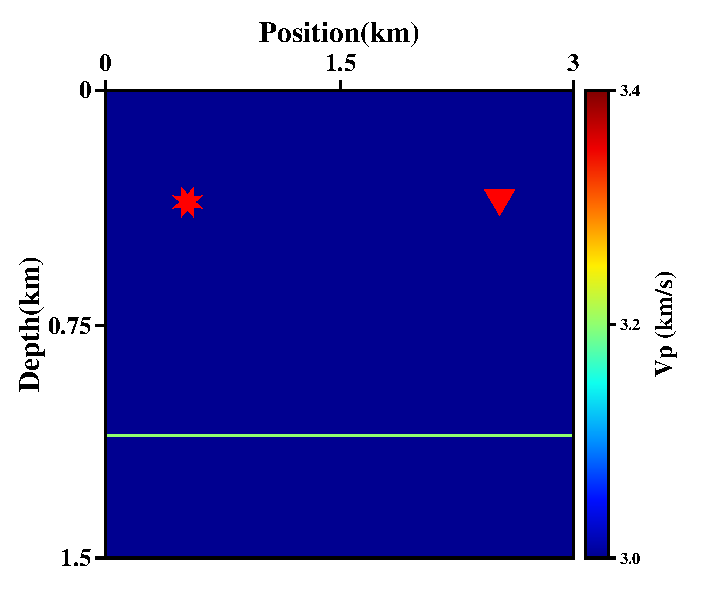
\includegraphics[width=0.30\textwidth]{Figure/chapter03/Kernel/1vp.pdf}}
   \subfloat[]{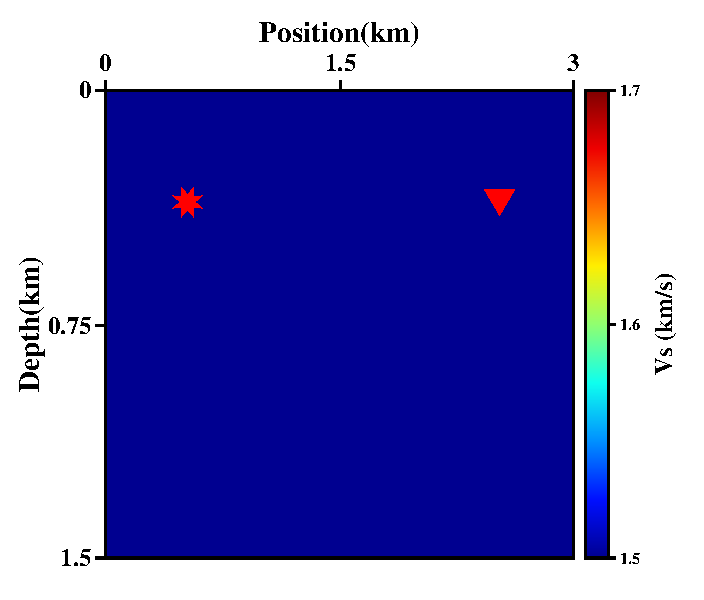
\includegraphics[width=0.30\textwidth]{Figure/chapter03/Kernel/1vs.pdf}}\\
   \subfloat[]{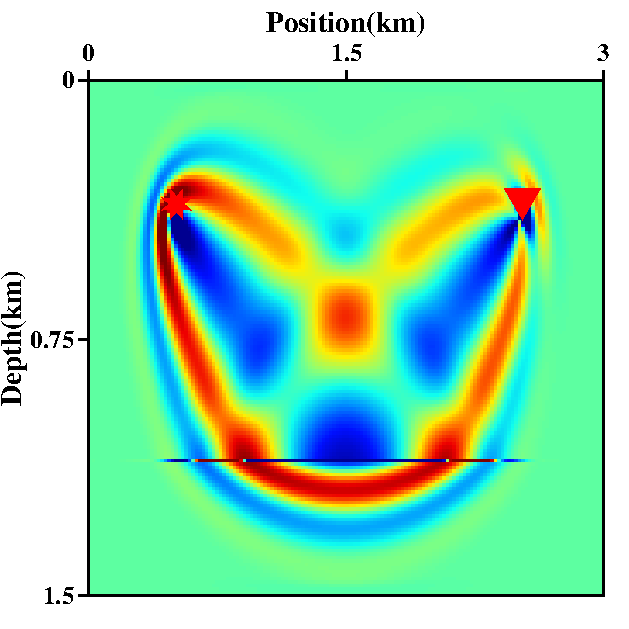
\includegraphics[width=0.30\textwidth]{Figure/chapter03/Kernel/Vponlyvp.pdf}}
   \subfloat[]{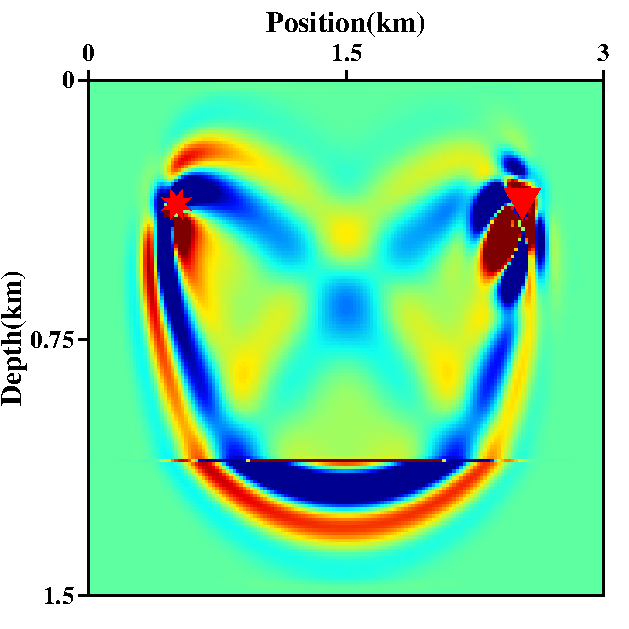
\includegraphics[width=0.30\textwidth]{Figure/chapter03/Kernel/Vsonlyvp.pdf}}\\
   \caption{单独$V_p$反射层时的反射波路径。(a)为$V_p$模型,(b)为$V_s$模型,(c)为$V_p$核函数,(d)为$V_s$核函数.}
   \label{fig:kernel1_vp}
\end{figure}

为了观察弹性波反射波路径核函数,我们在简单的单层界面中计算反射波波路径。首先,我们假定只有$V_p$的扰动界面,如图\ref{fig:kernel1_vp}(a), (b)
%\begin{figure}
%   \centering
%   \subfloat[]{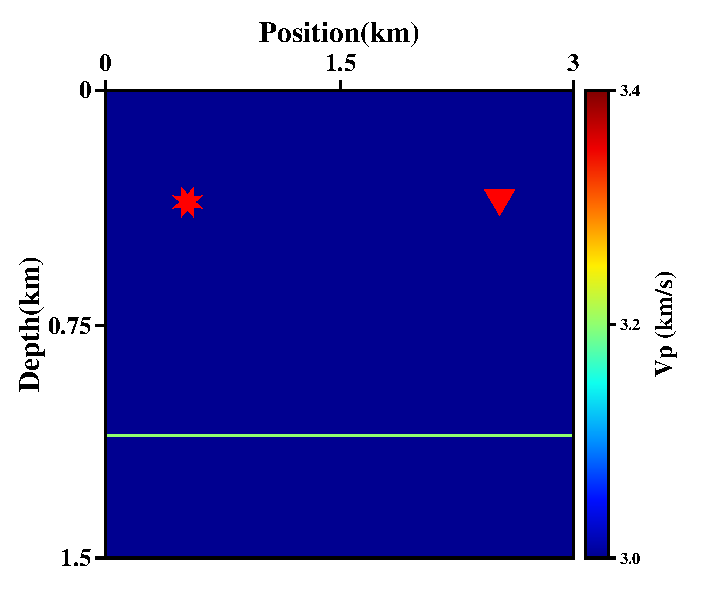
\includegraphics[width=0.38\textwidth]{Figure/chapter03/Kernel/1vp.pdf}}
%   \subfloat[]{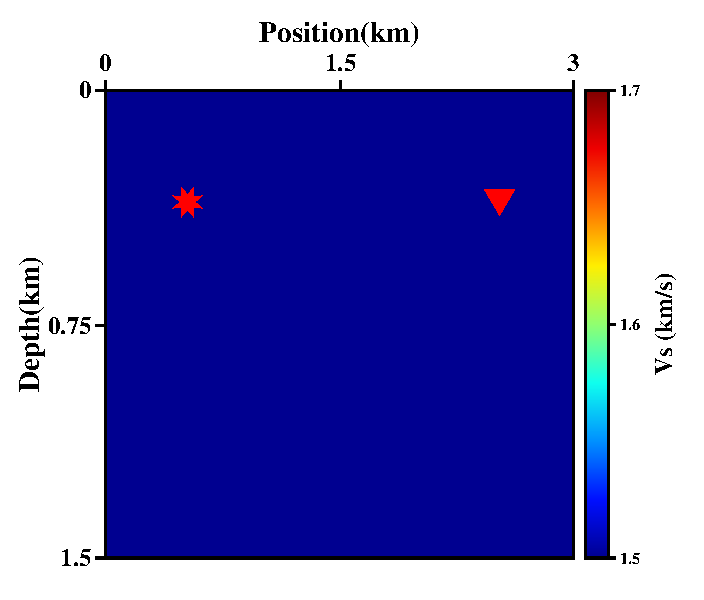
\includegraphics[width=0.38\textwidth]{Figure/chapter03/Kernel/1vs.pdf}}\\
%   \caption{单独$V_p$扰动界面。左侧为$V_p$,右侧为$V_s$.}
%   \label{fig:KernelModel1}
%\end{figure}
该模型由于没有$V_s$界面,因此没有模式转换能量只有PP波反射,非常接近于声波情况。
采用该模型获得的反射波波路径如图\ref{fig:kernel1_vp}(c)和(d)。可以看到,$V_p$的反射波
路径分为震源端以及检波点端左右两支,与声波波路径非常接近。同时$V_s$也会有相应的路径能量,但是路径中能量主要集中在边缘部分,中央第一菲涅尔带区域
能量较弱,可能的原因是这部分路径信息是由于PP波反射能量所产生,其对$V_s$背景信息并不敏感。
%如果换做$\lambda$和$\mu$的参数化方式,其产生的波路径如图\ref{Kernel1_lambda}所示
%\begin{figure}
%   \centering
%   \subfloat[]{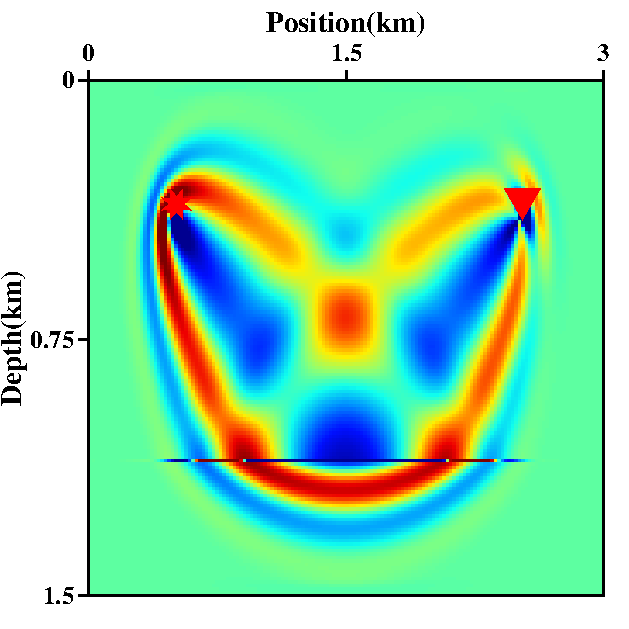
\includegraphics[width=0.30\textwidth]{Figure/chapter03/Kernel/lambdaonlyvp.pdf}}
%   \subfloat[]{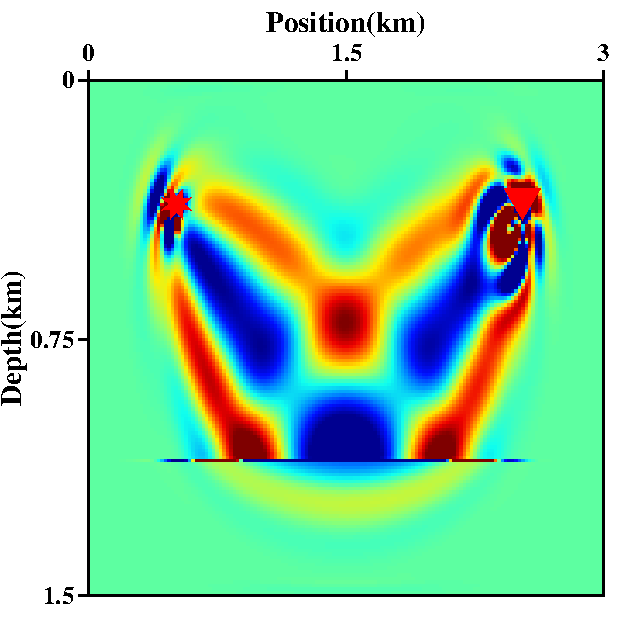
\includegraphics[width=0.30\textwidth]{Figure/chapter03/Kernel/muonlyvp.pdf}}\\
%   \caption{图\ref{fig:KernelModel1}模型$\lambda$参数化时的反射波路径。左侧为$\lambda$,右侧为$\mu$.}
%   \label{fig:kernel1_lambda}
%\end{figure}

之后,我们考虑$V_s$界面存在时的情况(图\ref{fig:kernel2}(a),(b)),这时波场就会变得十分复杂
,在正传及反传波场中会同时存在P波与S波,因此反射波路径将变得更加复杂,如图\ref{fig:kernel2})
\begin{figure}
   \centering
   \subfloat[]{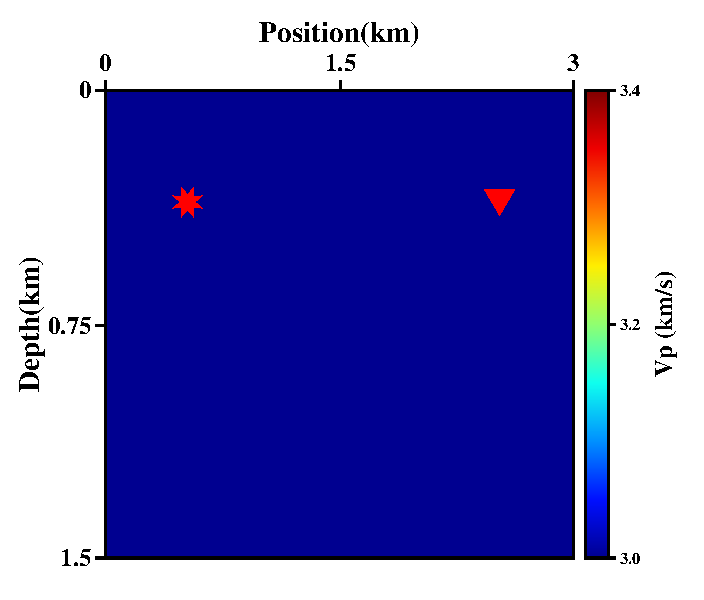
\includegraphics[width=0.30\textwidth]{Figure/chapter03/Kernel/2vp.pdf}}
   \subfloat[]{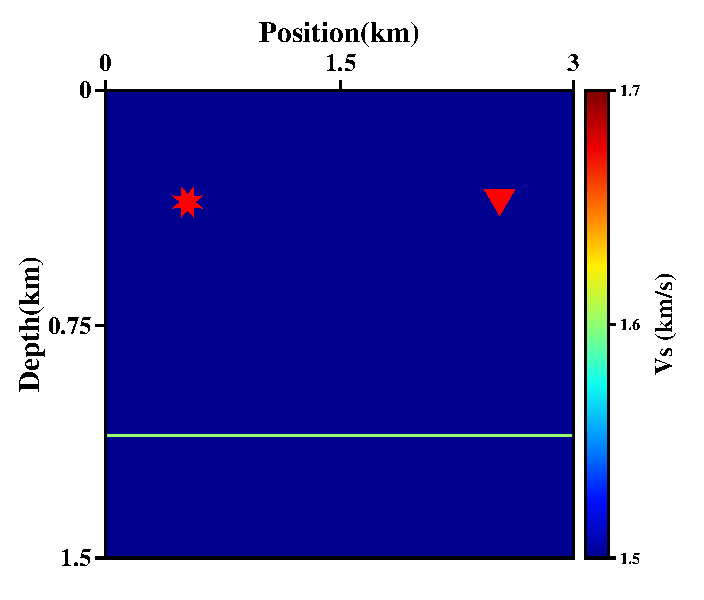
\includegraphics[width=0.30\textwidth]{Figure/chapter03/Kernel/2vs.pdf}}\\
   \subfloat[]{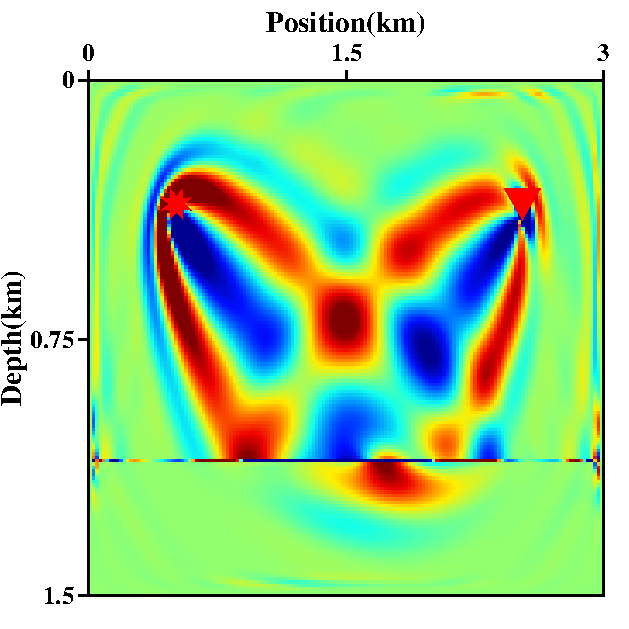
\includegraphics[width=0.30\textwidth]{Figure/chapter03/Kernel/Vponlyvs.pdf}}
   \subfloat[]{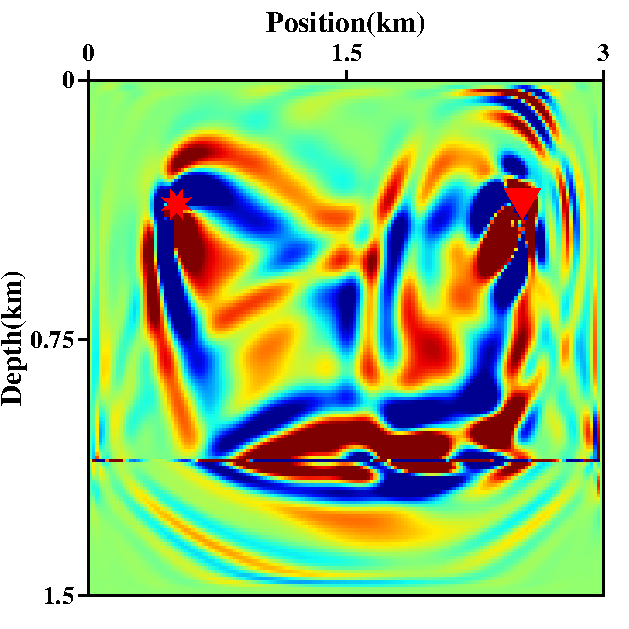
\includegraphics[width=0.30\textwidth]{Figure/chapter03/Kernel/Vsonlyvs.pdf}}\\
   \caption{单独$V_s$反射层时的反射波路径。(a)为$V_p$模型,(b)为$V_s$模型,(c)为$V_p$核函数,(d)为$V_s$核函数.}
%   \caption{单独$V_p$扰动界面。左侧为$V_p$,右侧为$V_s$.}
   \label{fig:kernel2}
\end{figure}
%\begin{figure}
%   \centering
%   \subfloat[]{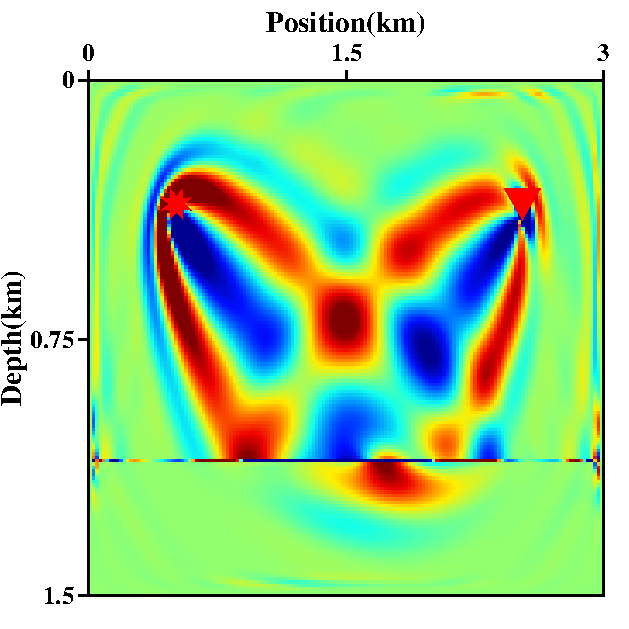
\includegraphics[width=0.30\textwidth]{Figure/chapter03/Kernel/Vponlyvs.pdf}}
%   \subfloat[]{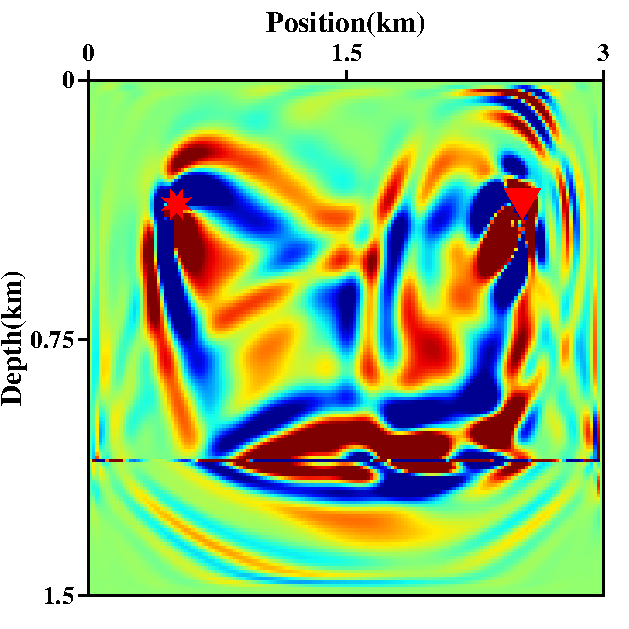
\includegraphics[width=0.30\textwidth]{Figure/chapter03/Kernel/Vsonlyvs.pdf}}\\
%   \caption{单独$V_p$扰动时的反射波路径。左侧为$V_p$,右侧为$V_s$.}
%   \label{fig:kernel2}
%\end{figure}
上图中,$V_p$核函数与图\ref{fig:kernel1_vp}中略有不同,这是因为由于存在$V_s$反射层,反传的散射波场在界面处产生“非物理”的S-P转换波,
这部分SP波与背景场中的P波互相关就会产生的一些假象。而在$V_s$的核函数中,可以看到多种模式转换导致的多个波路径叠加,使得核函数变得十分复杂。
尤其式其中的P波路径的能量总是占主导地位。
如果直接采用该核函数来计算$V_s$的梯度,一定会对反演带来更多的难度。根据式\ref{eq:decompkernel},我们将原始的$V_s$核函数分解为四个部分。
如图\ref{fig:kernel2_vs_decomp}所示,$K_{V_s}^{PP}$的能量与图\ref{fig:kernel2}c中
的$V_p$核函数十分类似,$K_{V_s}^{PS}$与$K_{V_s}^{SP}$则包含非常多的高频信息,
实际上它们是不同模式的正传与反传波场之间的偏移脉冲相应。而$K_{V_s}^{SS}$则与其他三者有些不同,其只包含了检波点端的一只反射路径,这是由于
我们采用了P波震源,在震源端的波场中不包含S波数据,因此$K_{V_s}^{SS}$的震源端项会是0。这样的话,$K_{V_s}^{SS}$就很少会受到P波路径的影响,这将
会非常有助于背景$V_s$的反演。
\begin{figure}
   \centering
   \subfloat[]{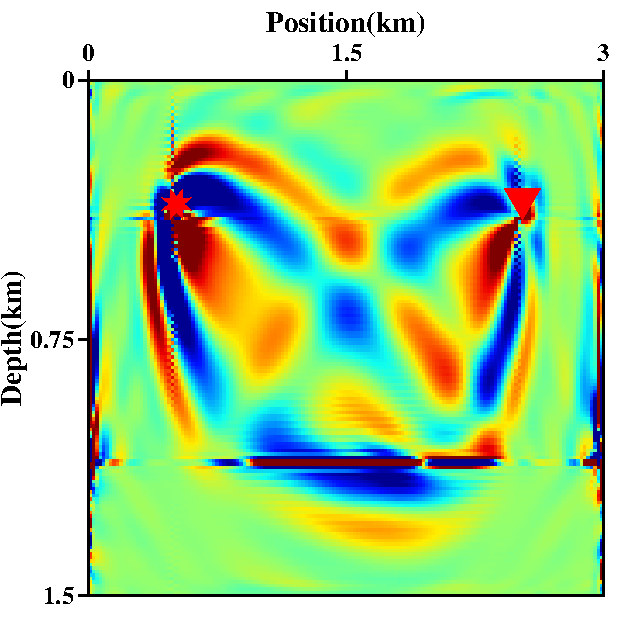
\includegraphics[width=0.30\textwidth]{Figure/chapter03/Kernel/VsonlyvsPP.pdf}}
   \subfloat[]{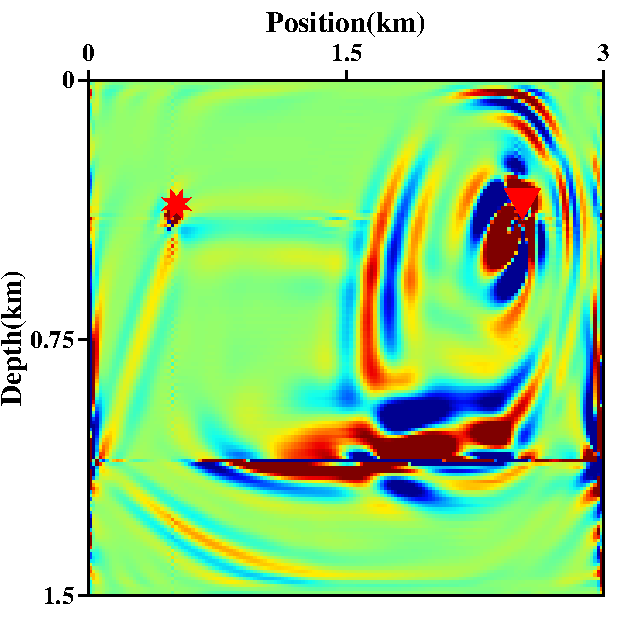
\includegraphics[width=0.30\textwidth]{Figure/chapter03/Kernel/VsonlyvsPS.pdf}}\\
   \subfloat[]{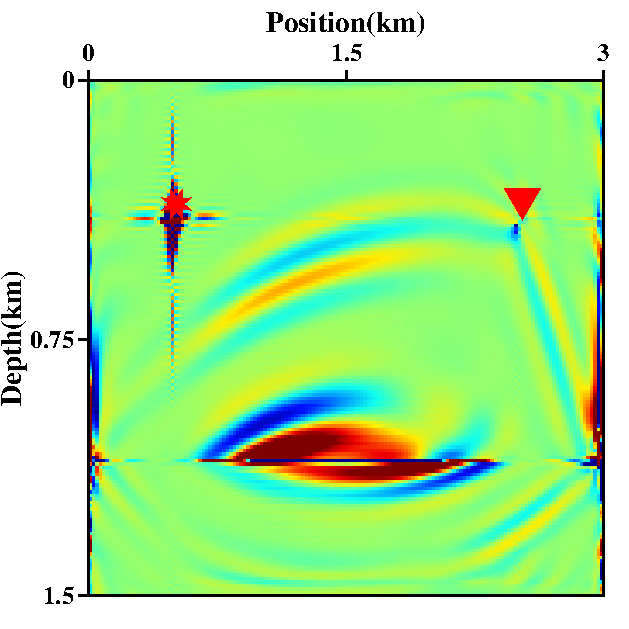
\includegraphics[width=0.30\textwidth]{Figure/chapter03/Kernel/VsonlyvsSP.pdf}}
   \subfloat[]{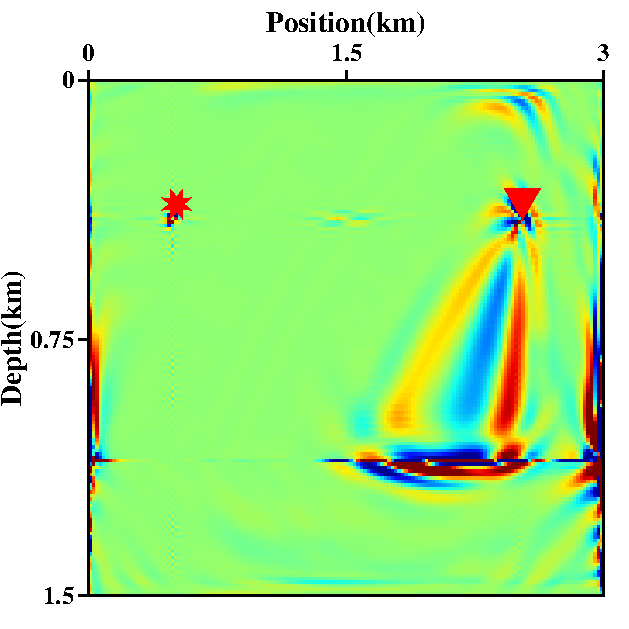
\includegraphics[width=0.30\textwidth]{Figure/chapter03/Kernel/VsonlyvsSS.pdf}}
   \caption{$K_{V_s}$核函数的四个分量。a, $K_{V_s}^{PP}$, (b) $K_{V_s}^{PS}$, (c) $K_{V_s}^{SP}$, (d) $K_{V_s}^{SS}$.}
   \label{fig:kernel2_vs_decomp}
\end{figure}
\section{弹性波WERTI工作流程}
弹性波介质中,不同模式的转换波,主要是PP与PS同相轴之间,会互相叠加、互相交叉。在用DIW提取走时差的时候,这些交叉点的位置就会变成一些奇异点而给拾取带来很大困难
。因此,如果直接用原始多分量数据的话,拾取到的$\tau(\mathbf{x_r},t;\mathbf{x_s})$就会不准确,这也是为什么式\eqref{eq:AdjointDeltaWE}中的梯度很难直接应用。
为了解决这个问题,我们将观测与模拟地震数据分解为P波与S波两部分。该模式分解只作用于地面地震数据\cite[]{Li2016a},因此我们可以快速地获得每一炮数据分解之后的矢量
P波或S波地震记录。这样,走时残差就可以被分成P波与S波两部分,使得弹性波WERTI变得可行,也即用一个两阶段的流程,先P波阶段后S波阶段。
\subsection{$V_p$反演}
在P波阶段,主要采用PP反射波来建立P波速度的背景模型。首先,我们从ERTM中获得P波速度的扰动,也即$\delta V_p$。
为了确保模拟的反射波与观测数据中的零(小)偏移距走时匹配,我们采用小偏移距的数据
获取$\delta V_p$。因为在速度不准的情况下大偏移距数据的偏移/反偏移结果会
造成模拟的反射波零偏移距走时变化,进而增加反演的困难程度。
此外,由于在WERTI中我们只考虑走时,所以我们只进行ERTM成像
而不是最小平方ERTM来拟合反射波振幅。
这也降低了反演中对反射系数估计的依赖程度。因此,目标函数变为最小化PP反射波的走时残差:
\begin{equation}
    E_{pp}=\frac{1}{2}\int\tau^2_{pp}(\mathbf{x_r},t;\mathbf{x_s})dtd\mathbf{x_r}d\mathbf{x_s}.
    \label{eq:ObjectivefunctionPP} 
\end{equation}
这样,采用P波记录来计算方程\eqref{eq:AdjointWE}的右端项,并用$\delta V_p$替换方程\eqref{eq:DeltaWE}和\eqref{eq:AdjointDeltaWE}中的$\delta c_{ijkl}$,我们
就可以计算得到$V_p$的梯度, $\frac{\partial E}{\partial V_p}$。与EFWI中一样,该梯度中的互相关项自动隐含了散度算子,因此,在
计算时只采用了PP波的反射波,所以模式解耦无法对该梯度起作用。

\subsection{$V_s$反演}
在S波阶段,我们将采用类似的策略但是只利用PS反射波。则目标函数变为:
\begin{equation}
    E_{ps}=\frac{1}{2}\int\tau^2_{ps}(\mathbf{x_r},t;\mathbf{x_s})dtd\mathbf{x_r}d\mathbf{x_s}.
    \label{eq:ObjectivefunctionPS} 
\end{equation}
但是,模拟PS反射波的实现方式与前一阶段策略略有不同。这里我们有两种思路来模拟PS反射波:

方式\uppercase\expandafter{\romannumeral1}: 采用反演好的$V_p$以及初始$V_s$模型来进行PS成像并使用该成像结果进行反偏移;

方式\uppercase\expandafter{\romannumeral2}: 由于$V_p$的背景速度已经获得了很好的恢复,此时PP波成像结果应该已经比较接近准确位置,且通常情况下,地
下介质中$V_p$与$V_s$的界面是比较一致的,因此也可以采用PP波成像结果。

但是经过测试,我们发现第一种方式产生的近偏移距走时
对$V_p$模型的误差非常敏感,即使$V_p$模型在真值附近也有可能获得错误方向的走时残差。
我们知道PS反射波的路径是非对称的,我们假定地下的简单PS反射路径如示意图\ref{fig:PS_refl}。
由几何关系以及snell定律,入射角$\theta_1$与反射角$\theta_2$之间以及深度、偏移距与该角度之间的关系为:
\begin{equation}
%\begin{split}
    \frac{sin\theta_1}{V_p}=\frac{sin\theta_2}{V_s},\qquad
    h(tan\theta_1+tan\theta_2)=X,
%\end{split}
    \label{eq:Snell_PS} 
\end{equation}
\begin{figure}
   \centering
   \subfloat{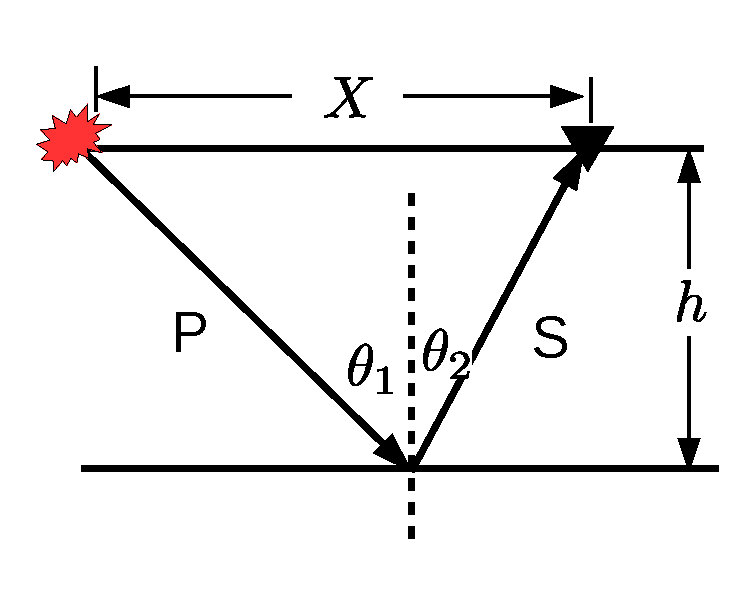
\includegraphics[width=0.40\textwidth]{Figure/chapter03/PS_problem/PS_refl.pdf}}
   \caption{单界面PS反射波示意图。}
   \label{fig:PS_refl}
\end{figure}
则该简单反射面的PS波时距曲线关系为:
\begin{equation}
	t=\frac{h}{cos\theta_1V_p}+\frac{h}{cos\theta_2V_s},
    \label{eq:TravelTime_PS} 
\end{equation}
在速度不准的时候我们通常先使用小偏移距数据进行偏移,获得界面之后反偏移获得模拟反射数据的走时,这个过程可以采用零(小)偏移距的图偏移+
式\ref{eq:TravelTime_PS}的正演来近似获得Born反射数据的时距关系。在图偏移过程中,零偏移距走时保持不变,则偏移后的深度位置满足:
\begin{equation}
	\frac{h^{'}}{V_p}+\frac{h^{'}}{V^{'}_s}=\frac{h}{V_p}+\frac{h}{V_s},
    \label{eq:Mapmigration_PS} 
\end{equation}
其中$V^{'}_p$和$V^{'}_s$为错误的偏移速度。可以求得:
\begin{equation}
	{h^{'}}=\frac{V^{'}_s(V_p+V_s)}{V_s(V^{'}_p+V^{'}_s)}h.
    \label{eq:ZerooffMig_PS} 
\end{equation}
通常情况下
$V_p>V_s$因此$\frac{V_p+V_s}{V^{'}_p+V^{'}_s}$中$V^{'}_p$的偏差也会带来很大的影响,
因此PS零偏移距成像界面的深度会同时受到$V_p$与$V_s$速度误差的影响。
我们将使用式\ref{eq:Snell_PS}-\ref{eq:ZerooffMig_PS}测试Born反射数据的时距关系对$V^{'}_p$和$h$的敏感性。
这里我们测试的参数为$V_p=2500m/s$, $V_s=1500m/s$, $V^{'}_s=1300m/s$, $V^{'}_p=2450-2550m/s$.
图\ref{fig:Sens_vp}中可以看到采用PS波偏移反偏移获取的Born反射数据对$V_p$的误差非常敏感,在$\pm50m/s$范围内就会引起反偏移数据的走时残差发生方向
改变,而如果采用PP波的偏移深度时,其更新方向都是正确的。
但也存在问题即在界面深度较深时,Born模拟的走时偏离真值较远,如果存在个同相轴就会难以进行震相间的匹配,这样即使DIW也会受到
cycle-skipping影响,但幸运的是界面深度较浅时,Born模拟走时与观测数据偏离并不远,这样的话可以层剥离的方式来解决深层反射的震相匹配问题。
\begin{figure}[h]
   \centering
   \subfloat[]{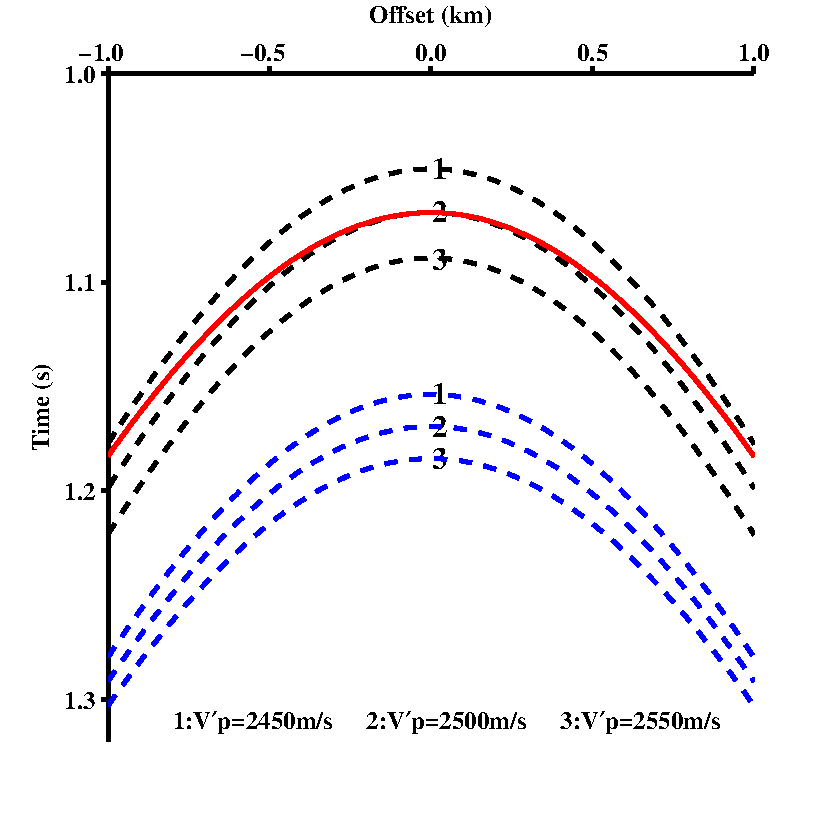
\includegraphics[width=0.48\textwidth]{Figure/chapter03/PS_problem/h1000.pdf}}
   \subfloat[]{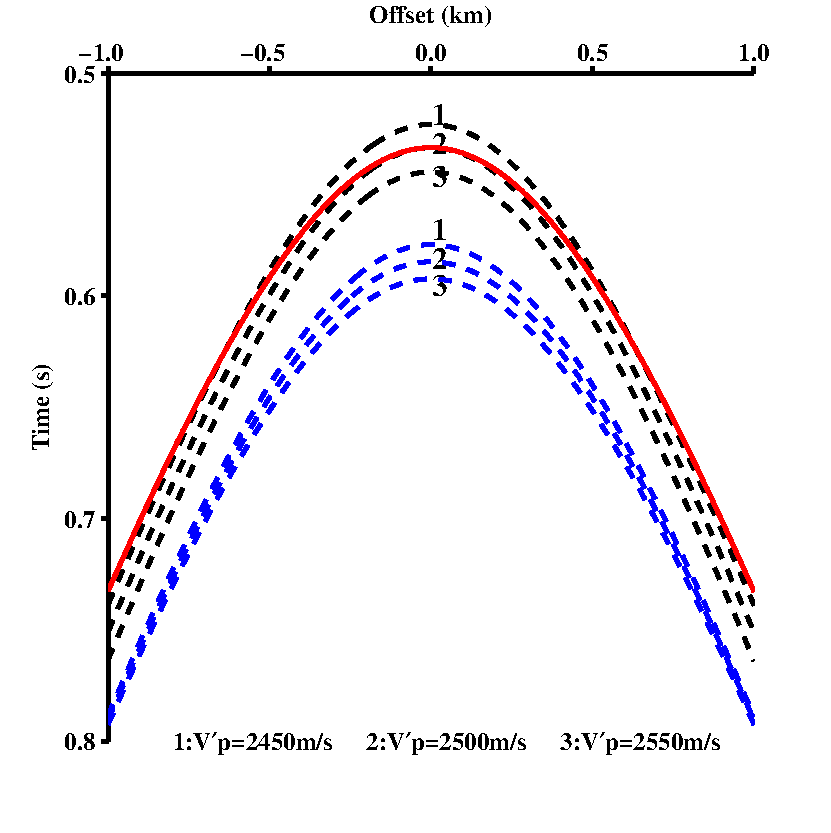
\includegraphics[width=0.48\textwidth]{Figure/chapter03/PS_problem/h500.pdf}}
   \caption{不同界面深度时方式\uppercase\expandafter{\romannumeral1}(黑色虚线)与
   方式\uppercase\expandafter{\romannumeral2}(蓝色虚线)反偏移获得PS波走时曲线
   与真实值(红色实线)之间的对比。数字1,2,3分别代表不同$V^{'}_p$速度的结果。(a) 界面深度$h=1000$; (b) 界面深度$h=500$.}
   \label{fig:Sens_vp}
\end{figure}

所以,我们推荐采用较为准确的PP成像($\delta V_p$)结果而不
是$\delta V_s$来产生PS反射波。这样做有两个弊端
第一、产生的PS反射无法保证振幅的准确性,但采用此种振幅不保真的同相轴并不会给DIW拾取走时残差带来非常大的
干扰。第二、来自深部的PS反射可能由于时差太大而受到cycle-skipping困扰,不过这个问题可以通过层剥离的方式,先更新浅层$V_s$
然后更新深层来避免。

此外,正如前文核函数分析提到,PS反射中,震源端波路径只与P波速度相关,
因此我们在计算$\frac{\partial E}{\partial V_s}$可以丢掉方程\eqref{eq:GradientCijkl} 
右端项的第一部分。并且,波模式分解也会施加在梯度的计算过程中来确保只有S波能量参与其中:
\begin{equation}
    \frac{\partial E_{ps}}{\partial V_s}=-2\rho V_s
    \int (\frac{\partial \delta u^S_{i}}{\partial
    x_j}\frac{\partial \psi^S_{k}}{\partial x_l})
    (\delta_{ik}\delta_{jl}+
    \delta_{il}\delta_{jk}).
    \label{eq:GradientVel}
\end{equation}
上述梯度与Wang et al. (2015)\cite{Wang2015a}提出的EFWI方法类似。模式解耦可以在$V_s$的反演中降低参数耦合同时也可以压制假象。

\section{局部倾角滤波约束}
WERTI非常类似成像域射线走时层析。而我们知道射线走时层析反问题通常不收敛,很难收敛或者很难收敛获得具有地质意义的模型。
在偏移后,成像结果可以提供地下界面大致的倾角信息,通过此类倾角信息,可以设计预条件算子来沿地层倾角来对反演进行约束,使得反演结果更合理。
采用倾角约束滤波可以加快收敛速度,在很大程度上改善反演结果。由于采用波动方程作为手段,WERTI采用波路径信息来反投影走时残差信息,因而其所面临的挑战要
小于射线走时层析。然而,对于一些照明不足,或者
反射路径覆盖不均匀的区域同样也会出现上述的问题。常规的各向同性的平滑算子很难保证反演收敛到具有地质含义的物理模型。因此,WERTI中采用局部倾角约束同样可以加速
收敛,并获得具有地质意义的反演结果。

Hale(2009)采用结构张量来估计地层倾角。对于2D的图像,结构张量是$2\times2$的矩阵:
\begin{equation}
        \mathbf{S}=
        \begin{pmatrix}
                < s^2_1 > \quad <s_1s_2 >\\
                < s_1s_2 > \quad < s^2_2 >\\
        \end{pmatrix},
        \label{eq:StructureTensor}
\end{equation}
其中$s_1$和$s_2$表示图像垂直和水平方向的方向导数,$<\dot>$表示2D的Gaussian平滑函数。上式对应的特征值问题可以表示为:
\begin{equation}
	\mathbf{S}=\lambda_u\mathbf{u}\mathbf{u}^T+\lambda_v\mathbf{v}\mathbf{v}^T
        \label{eq:EigenValueVector}
\end{equation}
其中,$\lambda_u$和$\lambda_v$分别为特征向量$\mathbf{u}$和$\mathbf{v}$对应的特征值。我们定义$\lambda_u\ge\lambda_v\ge0$,这样的话$\mathbf{u}$指示梯度最大的
方向,也即与线性结构垂直的方向。而话$\mathbf{u}$则指示与线性结构平行的方向。Hale(2009)指出,可以设置$\lambda_u(\mathbf{x})=0$
和$\lambda_v(\mathbf{x})=1$,这样保证图像中每一处平滑都会沿倾角方向。则沿倾角平滑的滤波器可以通过以下方程求解:
\begin{equation}
	(\mathbf{B}^T\mathbf{B}+\mathbf{A}^T\mathbf{S}^{\prime}\mathbf{A})\mathbf{h}=\mathbf{B}^T\mathbf{B}\mathbf{f}
        \label{eq:SparseMatrixSystem}
\end{equation}
其中,$\mathbf{S}^{\prime}$为新构造的结构张量,$\mathbf{B}$和$\mathbf{A}$分别为求和算子以及差分算子对应的矩阵,$\mathbf{f}$为输入图像,$\mathbf{h}$
为输出的平滑后图像。该方程可以通过共轭梯度法快速求解。

\section{数值实验}
\subsection{目标函数性态变化}
事实上,除了DIW提取走时之外,空间或者时间方向上的互相关也经常用来作为提取走时的方式\cite{vanLeeuwen:2010,chi2015,Wang2015},其目标函数为:
\begin{equation}
\left\{
	\begin{aligned}
		&\Delta t(h)=\mathop{\arg\min}_{\Delta t}\int d^{obs}(t+\Delta t,h)d^{cal}(t,h)dt,\\
	&E_t=\frac{1}{2}\sum\parallel \Delta t(h)\parallel ^2
	\end{aligned}
	\right.
    \label{eq:Obj_TimeCorr} 
\end{equation}
或
\begin{equation}
\left\{
	\begin{aligned}
		&\Delta h(t)=\mathop{\arg\min}_{\Delta h}\int d^{obs}(t,h+\Delta h)d^{cal}(t,h)dt,\\
	&E_h=\frac{1}{2}\sum\parallel \Delta h(t)\parallel ^2
	\end{aligned}
	\right.
    \label{eq:Obj_TimeCorr} 
\end{equation}
互相关提取的时差是每一道或每一时刻数据全局性的平均效果,
如果数据中反射同相轴比较多时,互相关反映出来的时差并不能体现某一个同相轴的趋势。这就导致如果在模型复杂的时候,很难应对多震相的问题。
而对比式\ref{eq:Objectivefunction}可以发现,DIW则衡量的是局部的数据差异,其更能反映局部的同相轴时差。这里我们将对比
在不同模型复杂程度下以上三种目标函数的性态变化。
由于给定了准确深度位置,PS波走时匹配需要采用层剥离逐步逼近,该过程较为复杂,因此我们这里只对PP波走时进行目标函数性态分析。我们采用常速背景+反射
系数的方式通过Born正演获得反射波观测数据,然后扰动背景速度,通过偏移/反偏移的方式计算目标函数值。

\begin{figure}
   \centering
   \subfloat[]{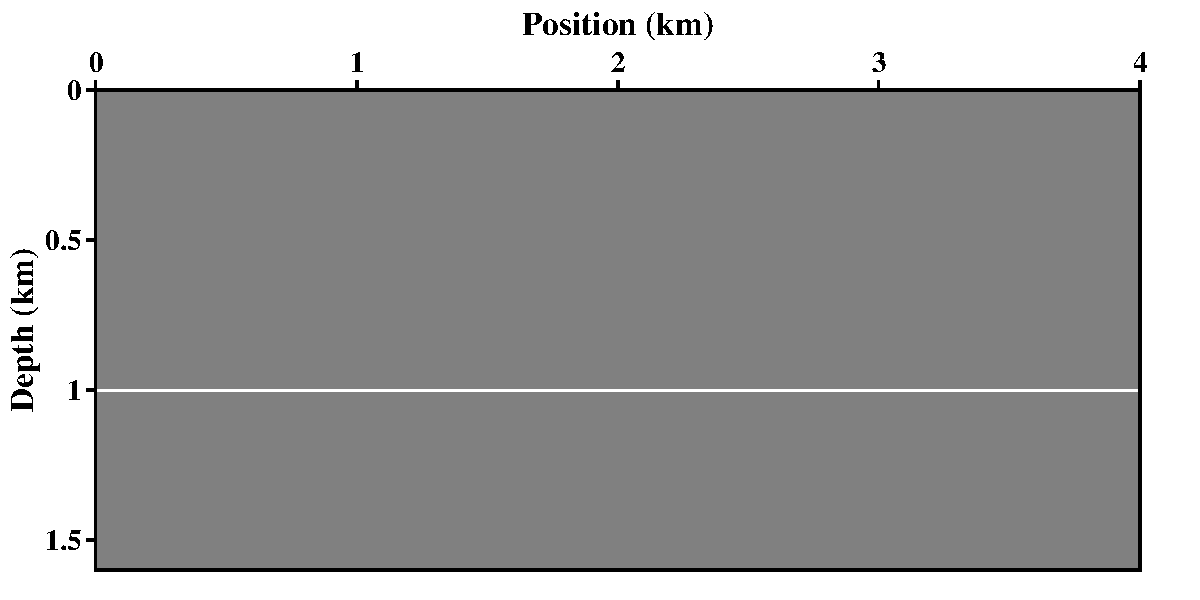
\includegraphics[width=0.48\textwidth]{Figure/chapter03/DIW_L2/1layer.pdf}}
   \subfloat[]{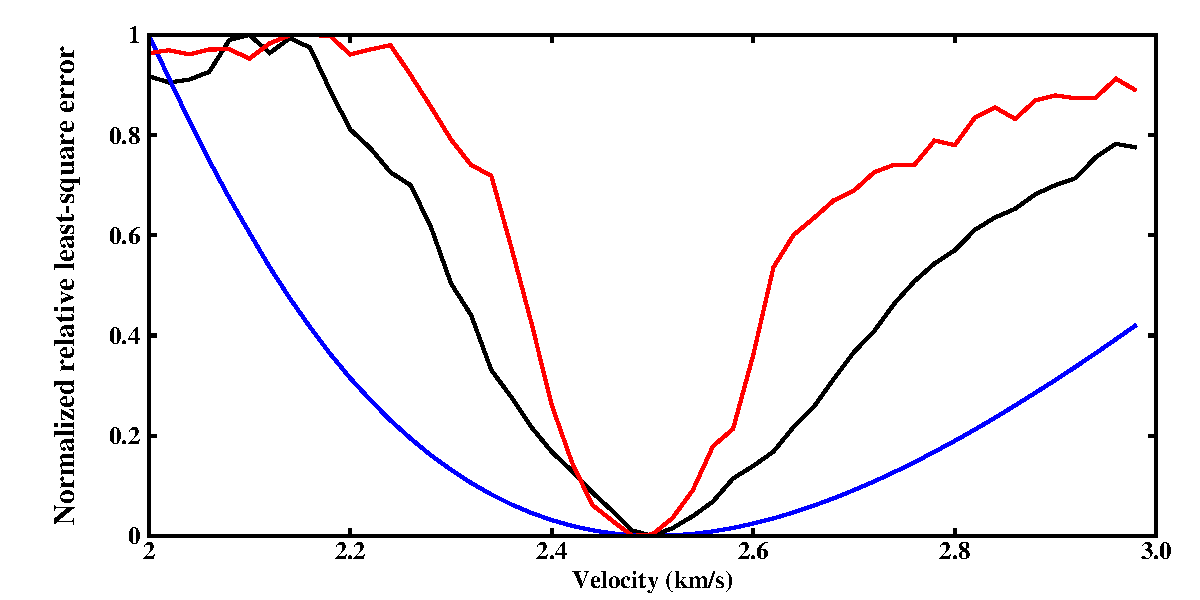
\includegraphics[width=0.48\textwidth]{Figure/chapter03/DIW_L2/1layerL2.pdf}}\\
   \subfloat[]{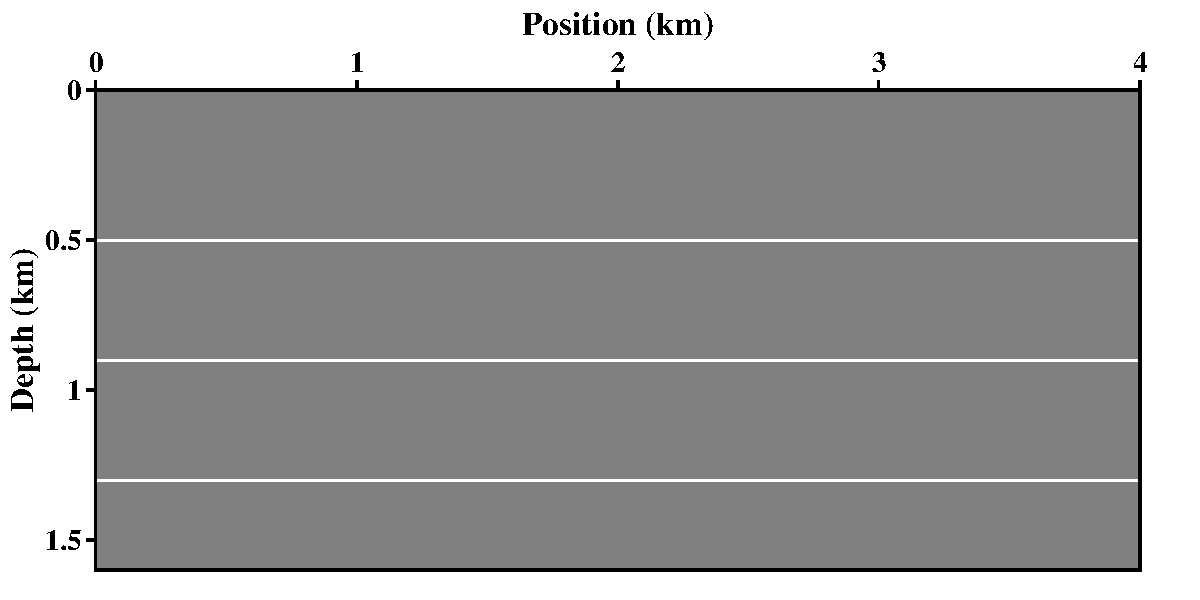
\includegraphics[width=0.48\textwidth]{Figure/chapter03/DIW_L2/3layer.pdf}}
   \subfloat[]{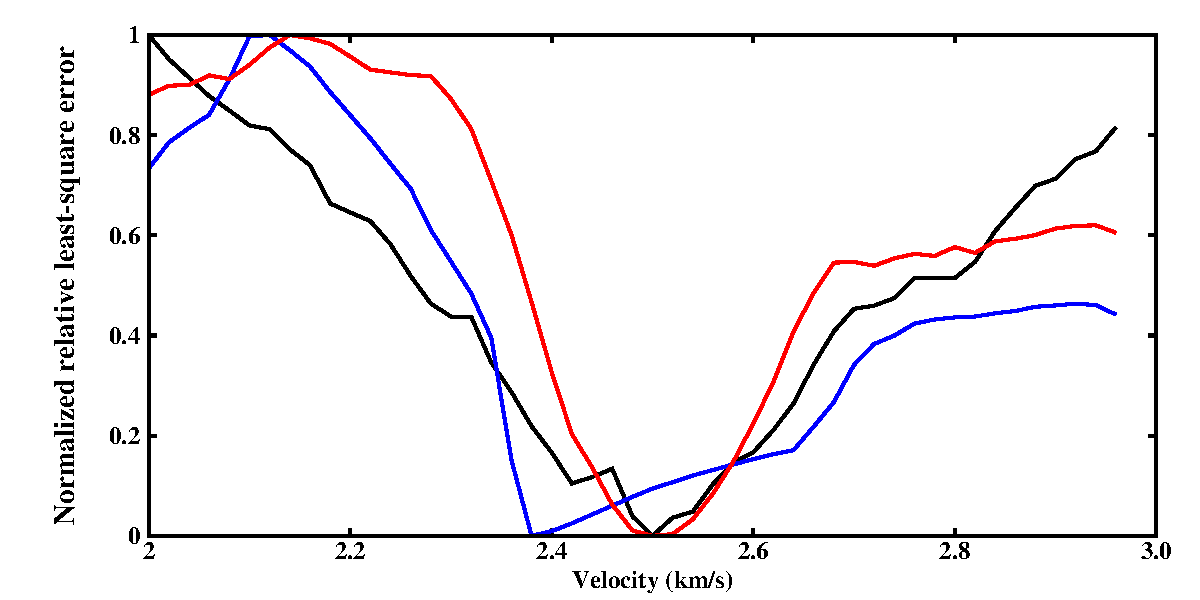
\includegraphics[width=0.48\textwidth]{Figure/chapter03/DIW_L2/3layerL2.pdf}}\\
   \subfloat[]{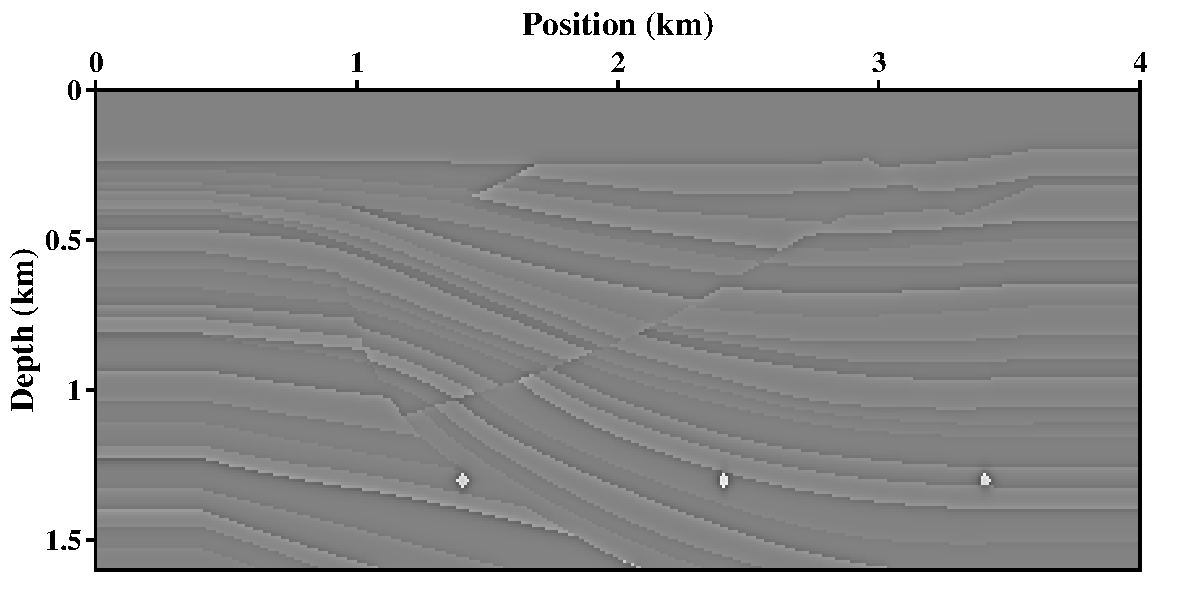
\includegraphics[width=0.48\textwidth]{Figure/chapter03/DIW_L2/Sigsbee.pdf}}
   \subfloat[]{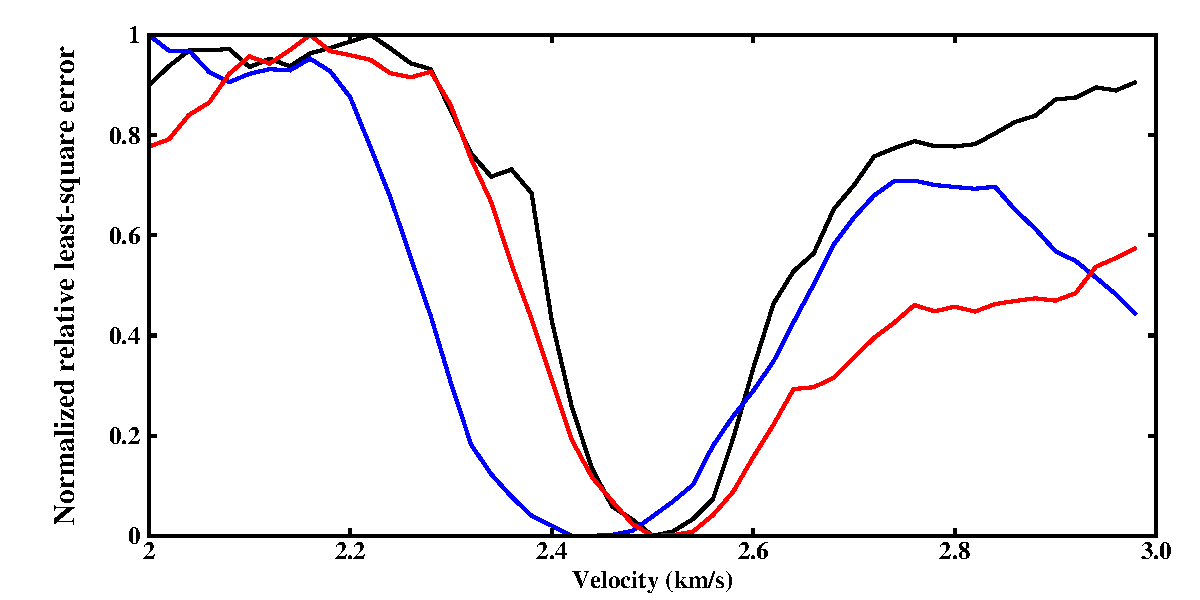
\includegraphics[width=0.48\textwidth]{Figure/chapter03/DIW_L2/complexL2.pdf}}
   \caption{不同模型及对应的PP波走时目标函数变化曲线。红色,蓝色和黑色分别对应DIW,时间互相关与空间互相关走时提取方式。}
   \label{fig:L2}
\end{figure}
三种不同模型对应的目标函数性态如图\ref{fig:L2}。
可以看到在单层界面时,反射同相轴单一可区分度很高,由于DIW为局部数据匹配,其计算也会受到cycle-skipping影响,
此时时间和空间互相关的目标函数表现要优于DIW。在三层模型中,由于反射同相轴变多,空间和时间互相关的目标函数准确性快速下降。空间互相关方式在
真值附近出现了局部极值。而时间互相关由于更难反映出时差随深度的变化,
其极值点出现在了错误的数值附近。但是DIW方式的稳定性并未随之剧烈变化,只是在速度偏大时对速度变化
不敏感,这也是由于受到cycle-skipping影响。
最后我们选取Sigsbee2A模型一部分的来做上述测试,
可以看到时间互相关目标函数的极值点仍然偏离准确值较远,
空间互相关目标函数也开始变得对初始模型更加敏感,而基于DIW的目标函数在复杂构造下仍然变化不大,可以说其收敛性相对更加稳健。

\subsection{Sigsbee2A模型}
为了验证算法的有效性,我们采用Sigsbee2A模型的一部分来进行实验(如图\ref{fig:TrueAndInitial}a和\ref{fig:TrueAndInitial}b)。
其中$V_s$模型通过固定的泊松比来产生。
图\ref{fig:TrueAndInitial}c和\ref{fig:TrueAndInitial}d展示了$V_p$和$V_s$的初始模型,
其速度值随深度线性增加。我们可以看到初始模型中,$V_p$比真实值偏低而$V_s$则偏高,
但这两者都偏离真实值很远。
观测数据模拟采用交错网格有限差分求解方程\ref{eq:WE_3}
水平和深度方向上空间采样均为16m,时间采样为1.2毫秒,接收时间为3.6s。
36个炮点均匀的分布在地表,检波点也布放在地表,最大偏移距为4km,震源子波主频为15Hz。本文实验中我们采用纯P波震源。
初始模型的成像结果
\begin{figure}[h]
   \centering
   \subfloat[]{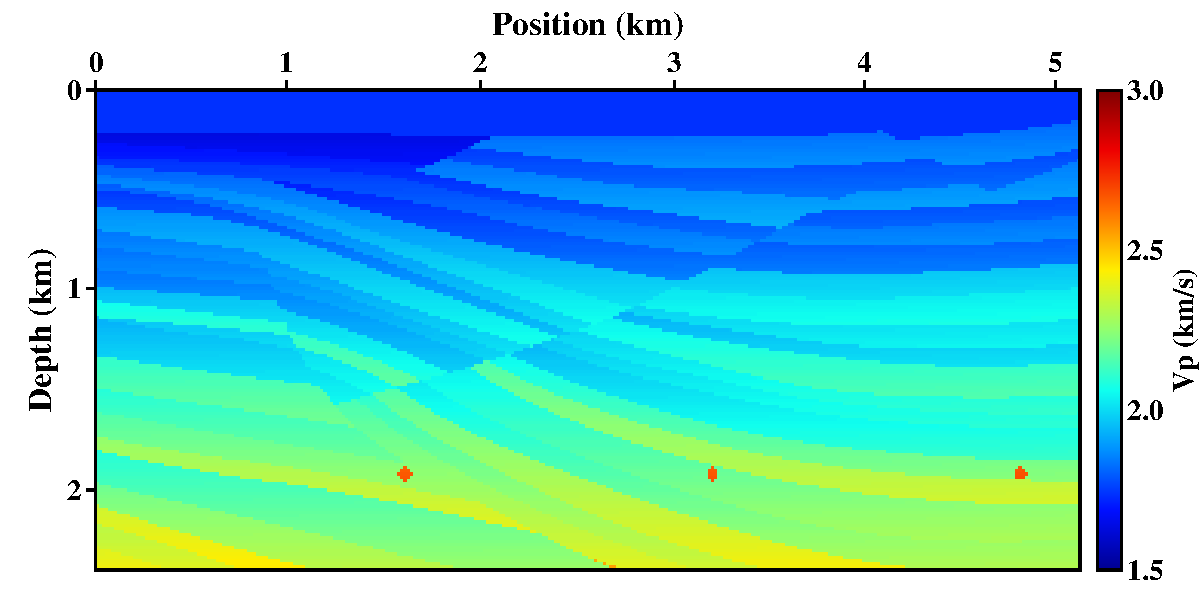
\includegraphics[width=0.48\textwidth]{Figure/chapter03/sigbee2/Fig/cuttruevp.pdf}}
   \subfloat[]{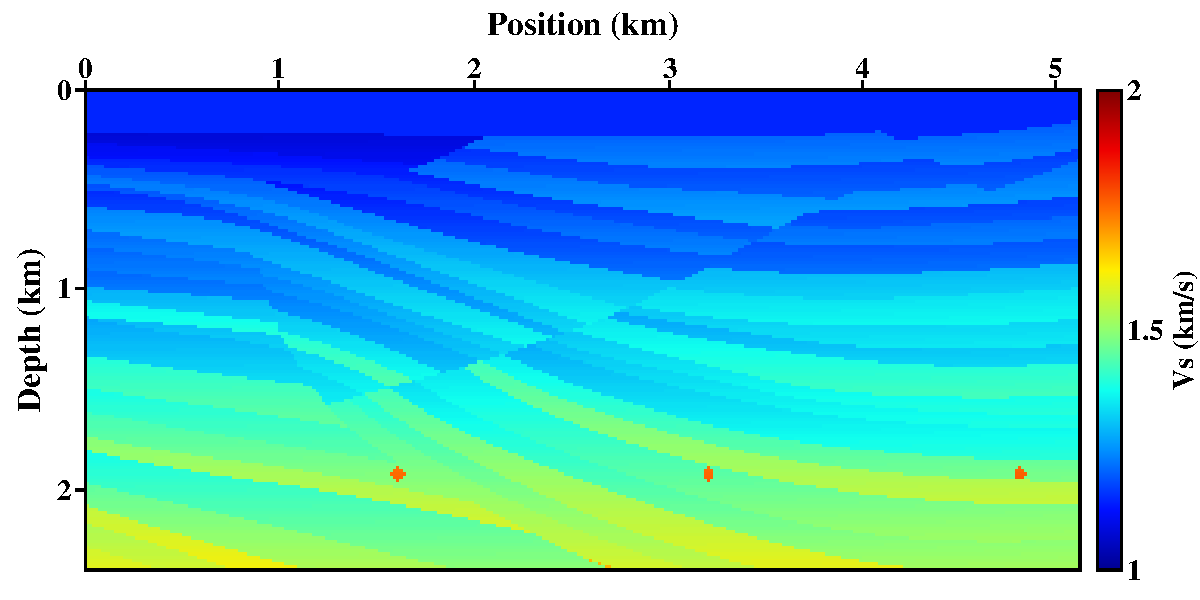
\includegraphics[width=0.48\textwidth]{Figure/chapter03/sigbee2/Fig/cuttruevs.pdf}}\\
   \subfloat[]{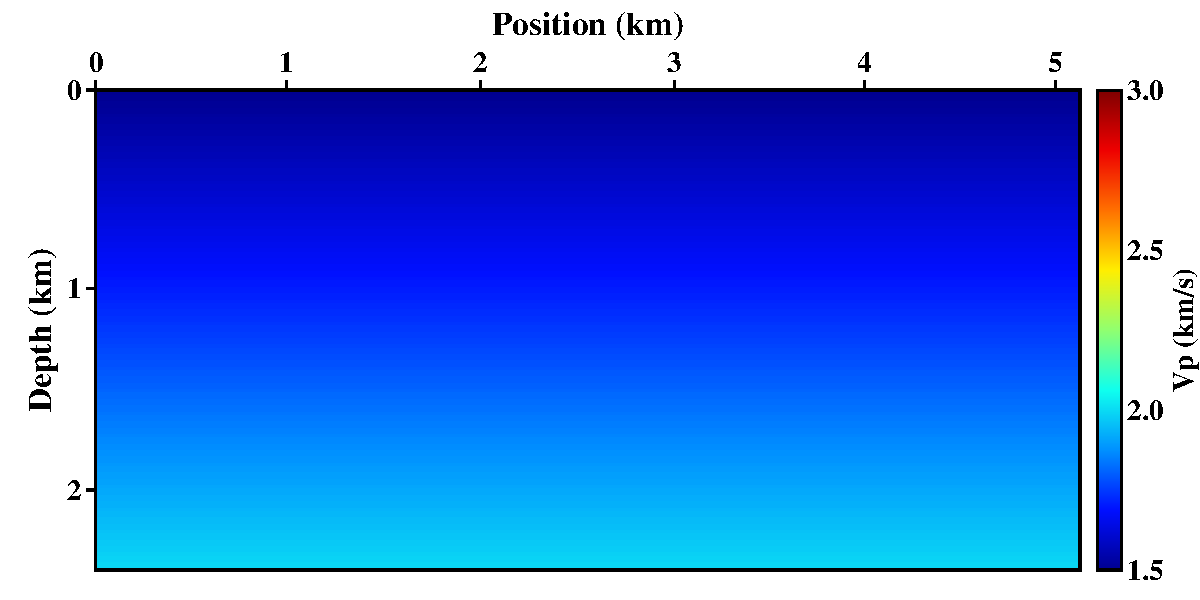
\includegraphics[width=0.48\textwidth]{Figure/chapter03/sigbee2/Fig/cutinitvp.pdf}}
   \subfloat[]{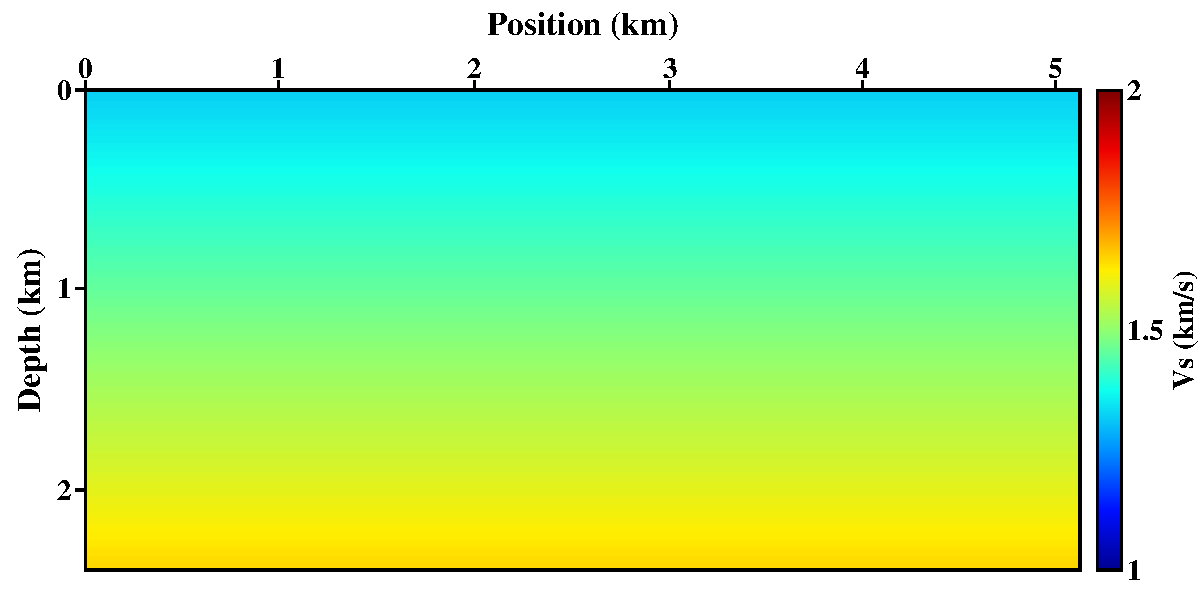
\includegraphics[width=0.48\textwidth]{Figure/chapter03/sigbee2/Fig/cutinitvs.pdf}}
   \caption{Sigbee2A真实$V_p$(a)和$V_s$(b)模型与初始$V_p$ (c)和$V_s$(d)模型。}
   \label{fig:TrueAndInitial}
\end{figure}

由于我们采用的初始模型随深度线性增大,其偏离真实值较远。
图\ref{fig:Results_init}为初始模型ERTM与EFWI结果。可以看到小偏移距ERTM成像结果界面位置全部错位,绕射波没有收敛。
PP与PS波成像结果都无法估计准确反射界面位置。如果采用该初始模型进行EFWI,
在浅部区域由于透射波存在还能够恢复出部分结构,但是随着深度的增加,由于速度中低波数成分不正确导致cycle-skipping存在,EFWI很快就会
陷入局部极值。
\begin{figure}[!htb]
   \centering
   \subfloat[]{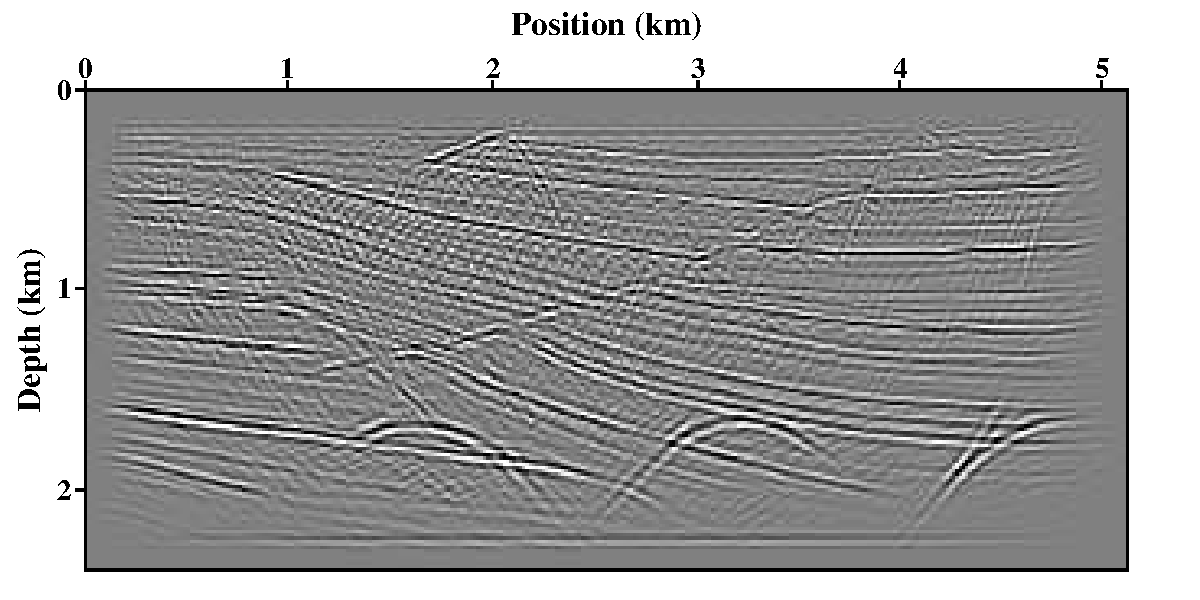
\includegraphics[width=0.48\textwidth]{Figure/chapter03/sigbee2/Fig/cutimage_initvp.pdf}}
   \subfloat[]{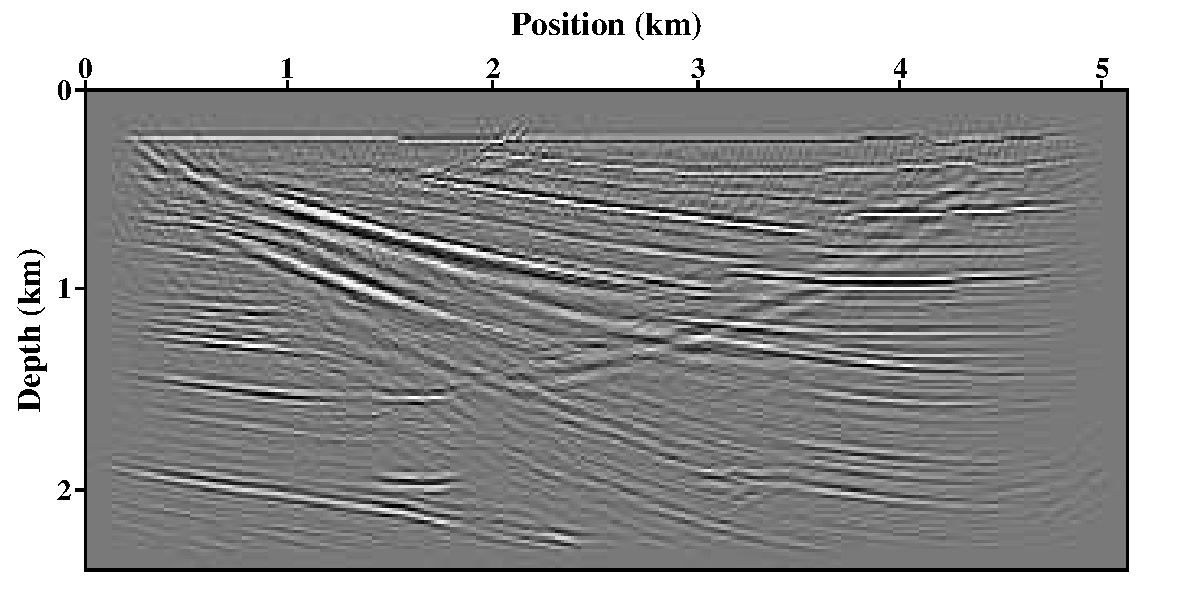
\includegraphics[width=0.48\textwidth]{Figure/chapter03/sigbee2/Fig/cutimage_initvs.pdf}}\\
   \subfloat[]{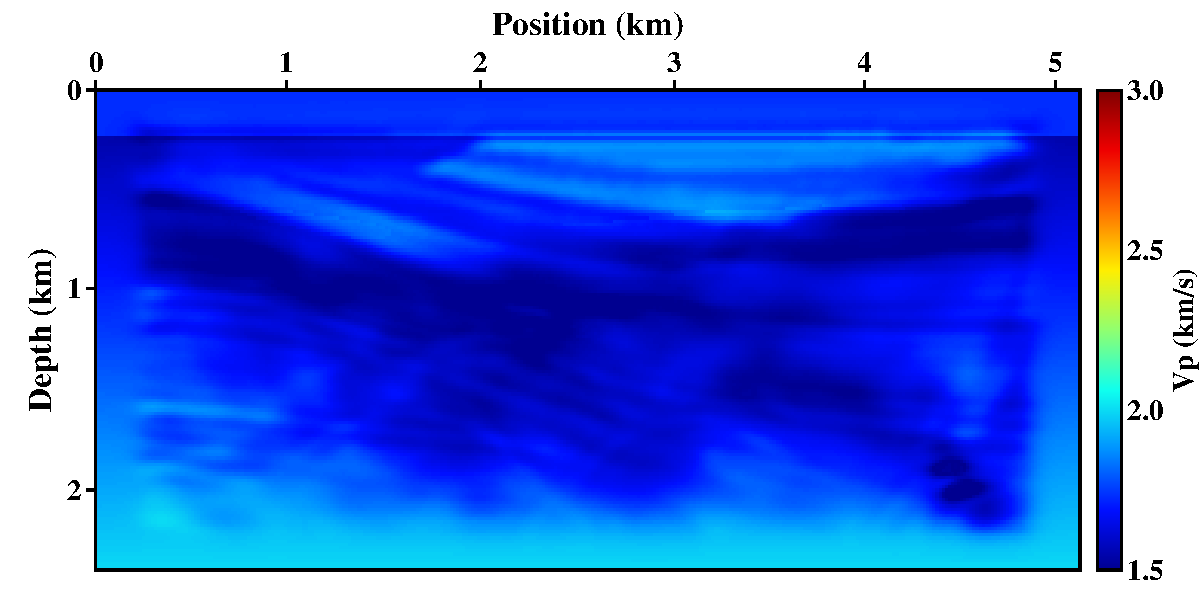
\includegraphics[width=0.48\textwidth]{Figure/chapter03/sigbee2/badinitvp.pdf}}
   \subfloat[]{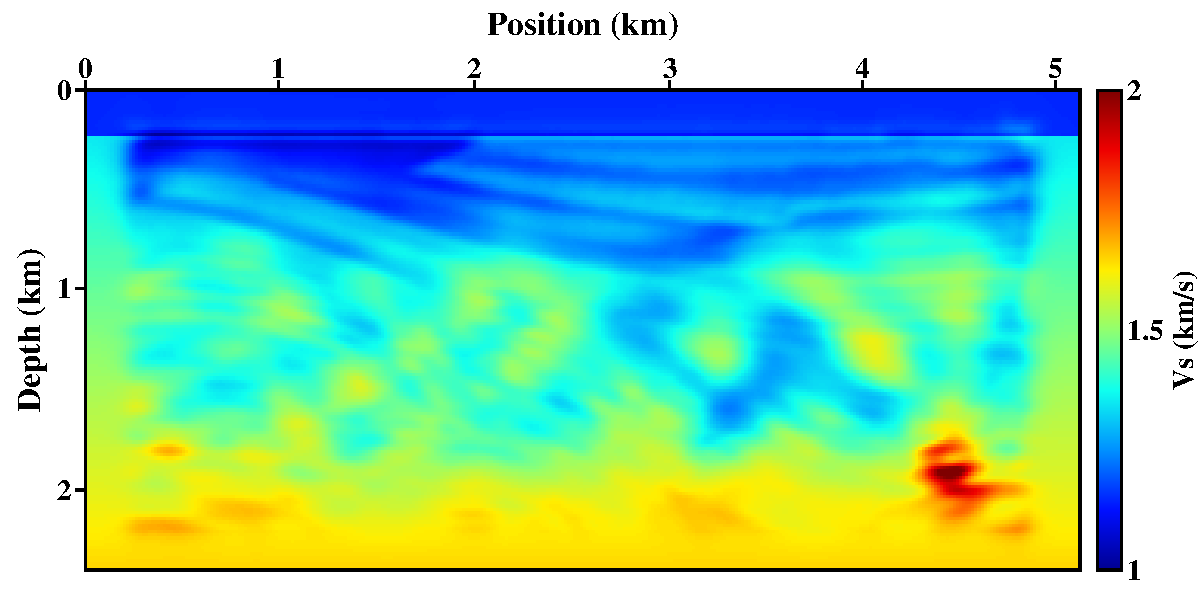
\includegraphics[width=0.48\textwidth]{Figure/chapter03/sigbee2/badinitvs.pdf}}\\
   \caption{初始模型下的小偏移距成像结果以及EFWI结果。(a)和(b)分别为PP与PS波ERTM结果,(c)和(d)分别为EFWI后$V_p$与$V_s$}
   \label{fig:Results_init}
\end{figure}

从上述糟糕的初始模型出发,我们按照前文所设计的工作流程进行E-WERTI,其反演结果如
图\ref{fig:InvertedModel}a和\ref{fig:InvertedModel}b为弹性WERTI的反演结果。
在经过每个阶段40次迭代之后,WERTI恢复了模型中深部的中低波数成分,但是对模型两侧反射数据覆盖较少以及最底部无反射波穿过的区域,
E-WERTI也无法反演。
\begin{figure}[!htb]
   \centering
   \subfloat[]{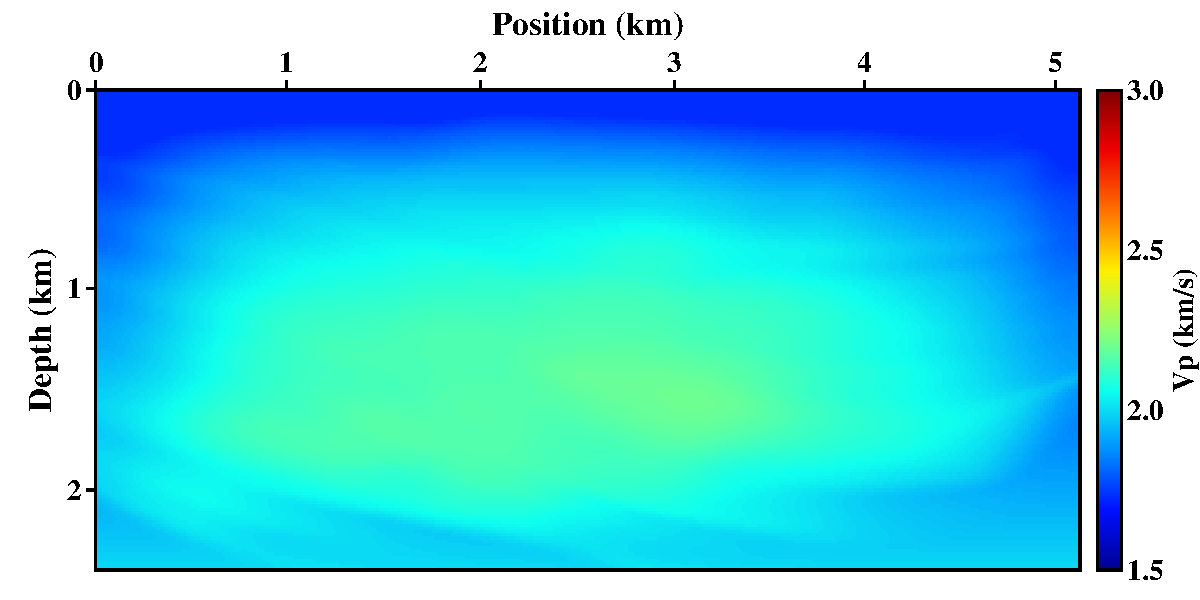
\includegraphics[width=0.48\textwidth]{Figure/chapter03/sigbee2/Fig/newinit3vp.pdf}}
   \subfloat[]{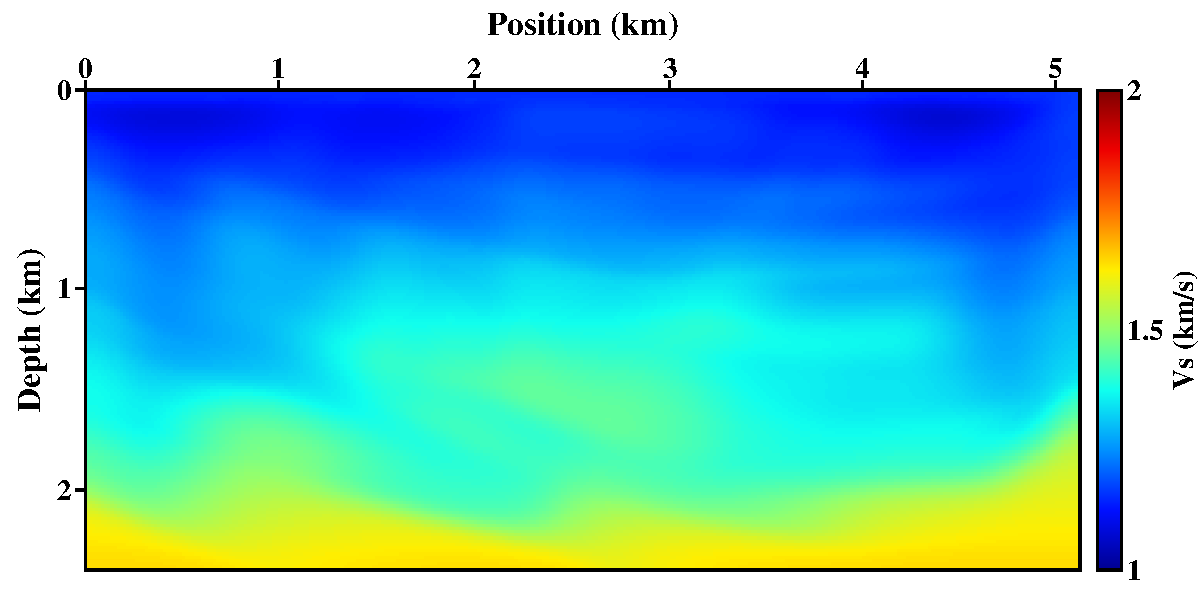
\includegraphics[width=0.48\textwidth]{Figure/chapter03/sigbee2/Fig/newinit3vs.pdf}}\\
   \caption{E-WERTI反演模型。(a) $V_p$, (b) $V_s$.}
   \label{fig:InvertedModel}
\end{figure}

采用上述模型我们重新进行ERTM成像,可以看到,随着模型中深部波数成分的恢复,PP波与PS波的成像结果得到了很大的改善,绕射波也得到了收敛。但在模型右侧
部分由于界面倾角以及观测数据限制,反射波接收补充分,E-WERTI未能很好地恢复模型中低波数成分,成像结果不是十分聚焦。
\begin{figure}[!htb]
   \centering
   \subfloat[]{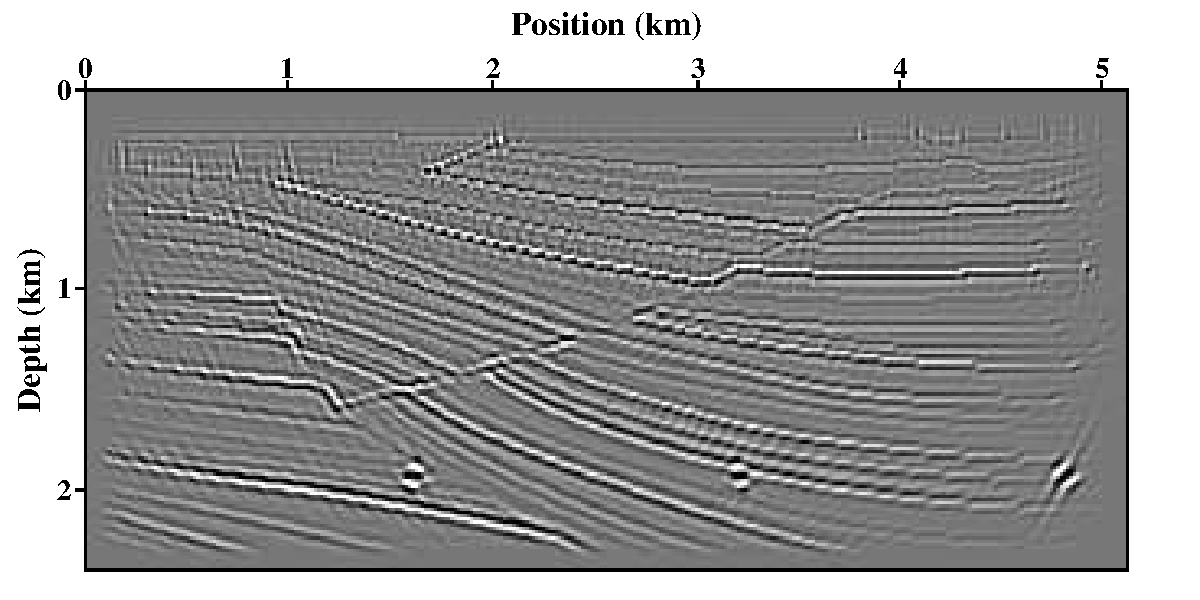
\includegraphics[width=0.48\textwidth]{Figure/chapter03/sigbee2/Fig/cutimage_truevp.pdf}}
   \subfloat[]{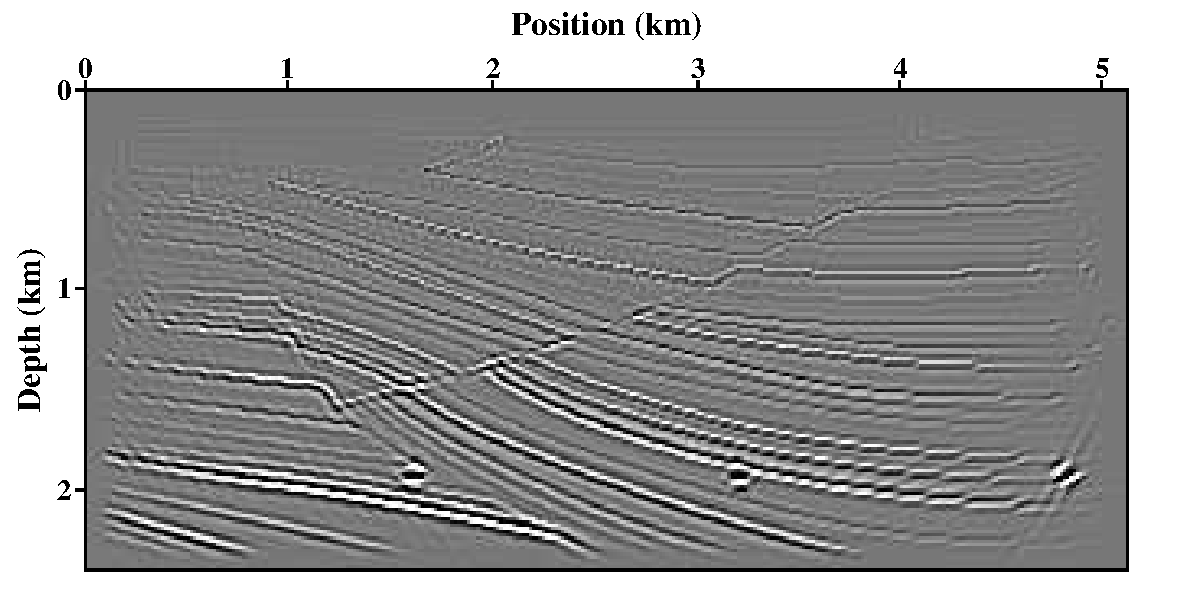
\includegraphics[width=0.48\textwidth]{Figure/chapter03/sigbee2/Fig/cutimage_truevs.pdf}}\\
   \subfloat[]{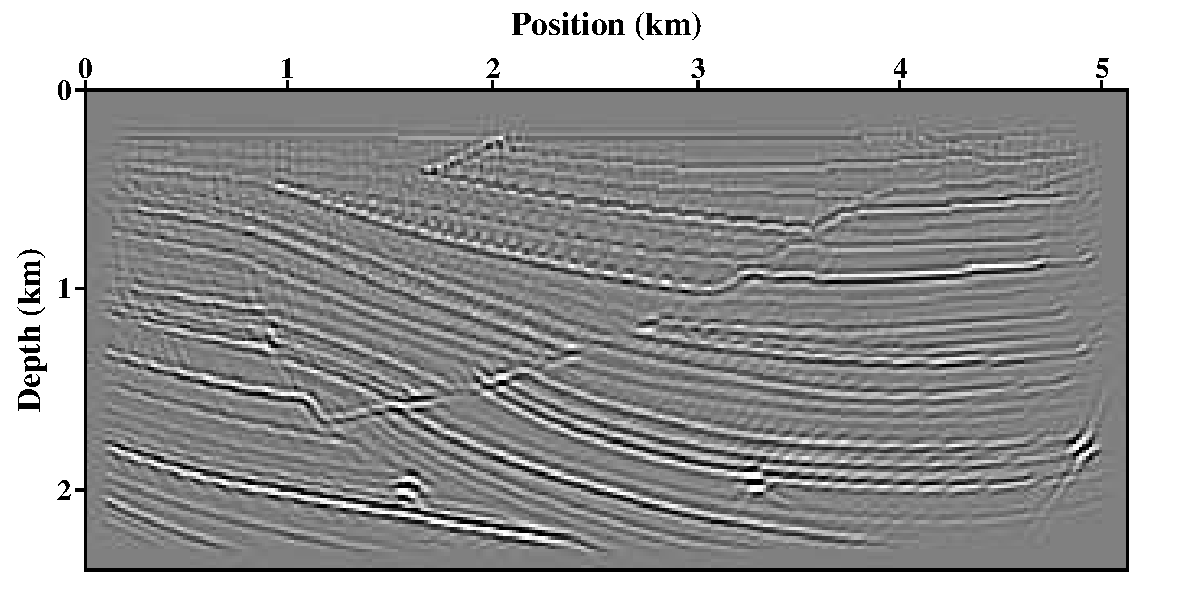
\includegraphics[width=0.48\textwidth]{Figure/chapter03/sigbee2/Fig/cutimage_wertivp.pdf}}
   \subfloat[]{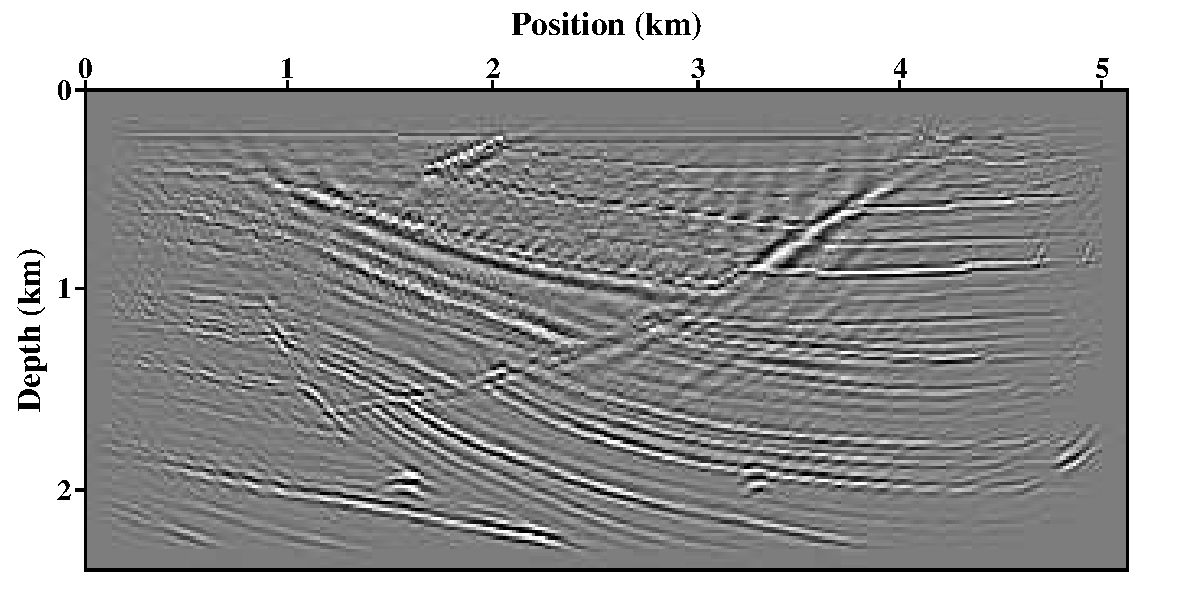
\includegraphics[width=0.48\textwidth]{Figure/chapter03/sigbee2/Fig/cutimage_wertivs.pdf}}
   \caption{真实模型与E-WERTI反演模型的ERTM结果对比。(a)和(b)分别为真实模型PP与PS波ERTM结果;(c)和(d)分别为E-WERTI模型PP与PS波ERTM结果。}
   \label{fig:ERTM_comparison}
\end{figure}
此外,我们也将E-WERTI前后的反射数据进行了对比。
\begin{figure}[!htb]
   \centering
   \subfloat[]{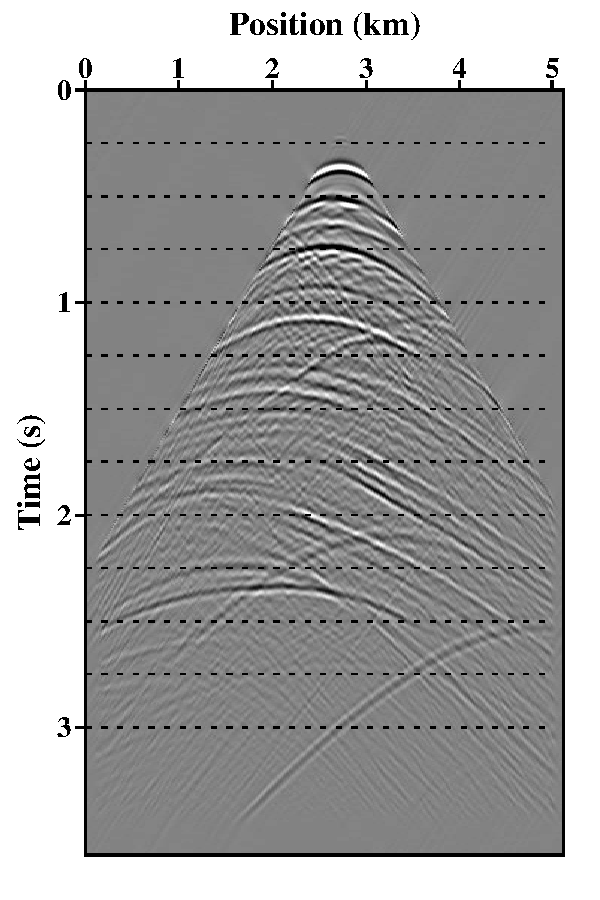
\includegraphics[width=0.33\textwidth]{Figure/chapter03/sigbee2/Fig/DataPP_true.pdf}}
   \subfloat[]{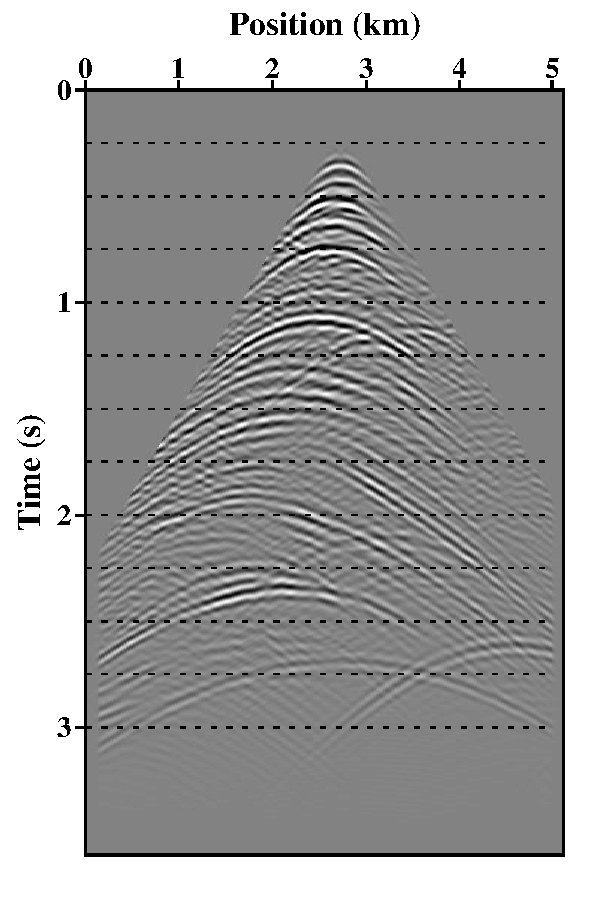
\includegraphics[width=0.33\textwidth]{Figure/chapter03/sigbee2/Fig/DataPP_init.pdf}}
   \subfloat[]{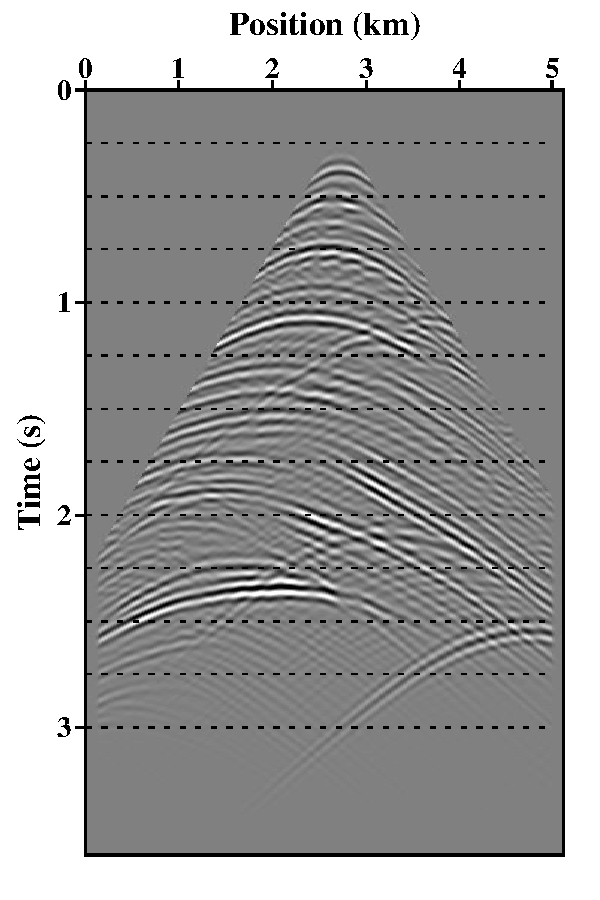
\includegraphics[width=0.33\textwidth]{Figure/chapter03/sigbee2/Fig/DataPP_werti.pdf}}\\
   \subfloat[]{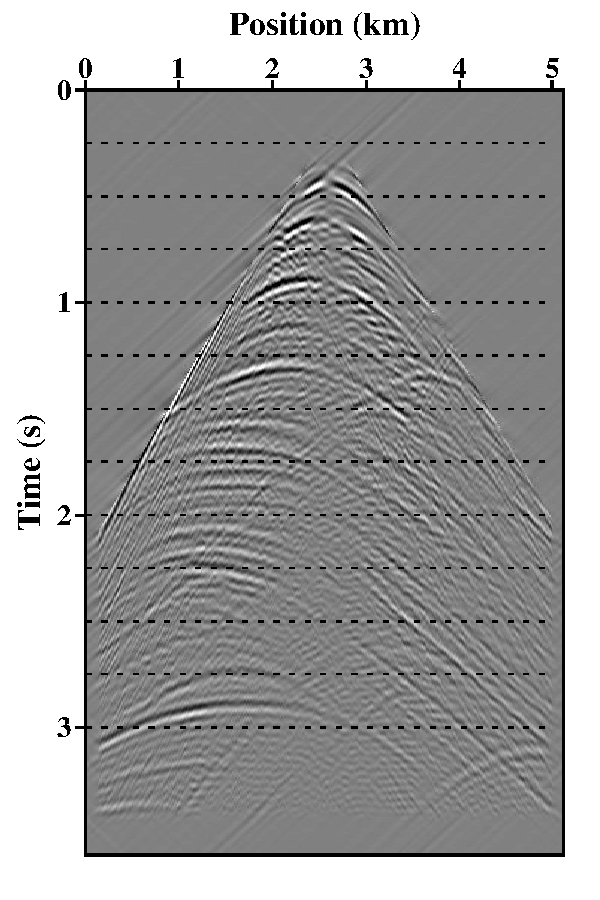
\includegraphics[width=0.33\textwidth]{Figure/chapter03/sigbee2/Fig/DataPS_true.pdf}}
   \subfloat[]{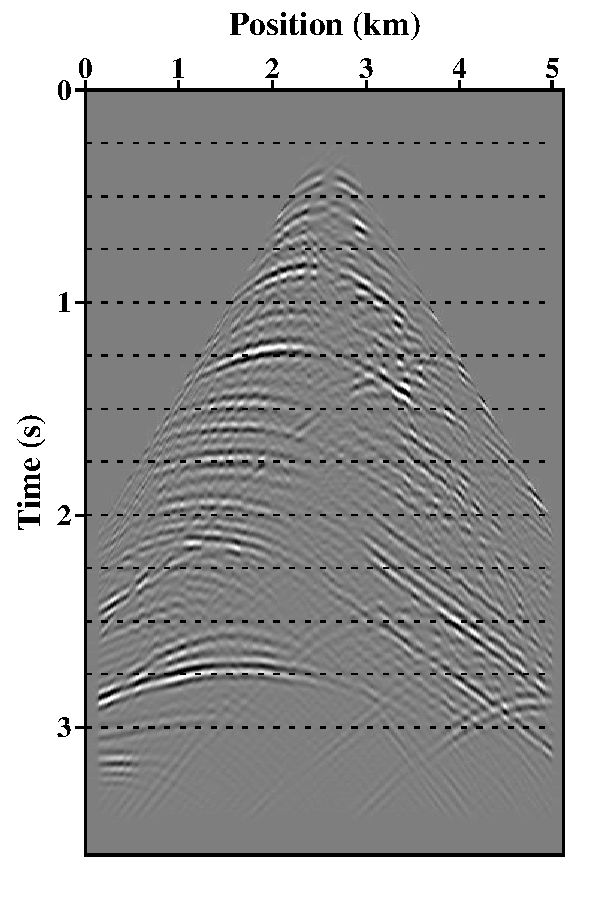
\includegraphics[width=0.33\textwidth]{Figure/chapter03/sigbee2/Fig/DataPS_init.pdf}}
   \subfloat[]{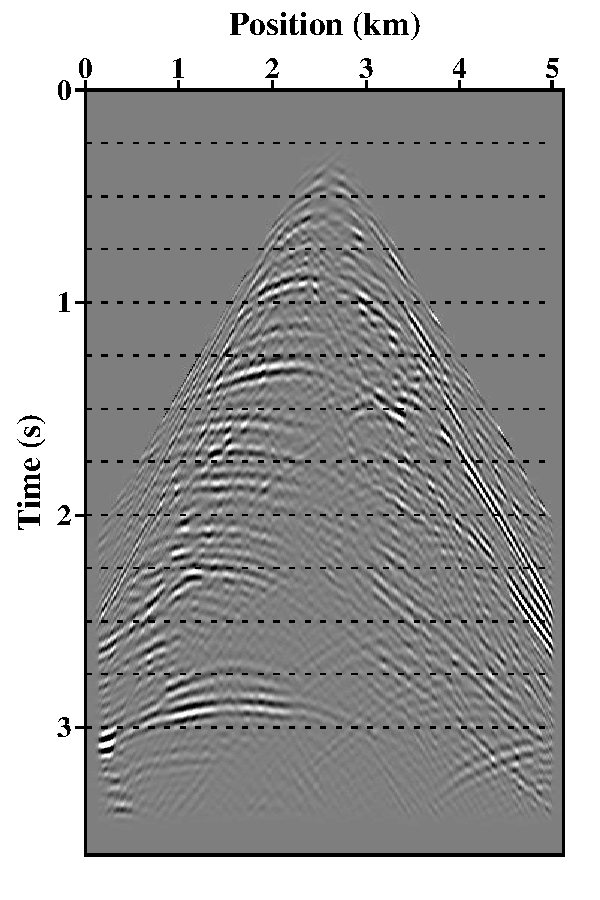
\includegraphics[width=0.33\textwidth]{Figure/chapter03/sigbee2/Fig/DataPS_werti.pdf}}
   \caption{真实反射数据(左),初始模型Born反射数据(中)与E-WERTI之后Born反射数据(右)之间的比较。(a),(b)和(c)为垂直分量,(d),(e),(f)为水平
   分量。}
   \label{fig:Data_comparison}
\end{figure}

上述结果中,局部倾角滤波约束对降低反演的多解性有着至关重要的作用。
在E-WERTI过程中,每次迭代的梯度我们都采用该轮迭代中的ERTM成像结果来进行局部倾角滤波约束。从图\ref{fig:LSF_comparison}b中可以看到,
尽管E-WERTI的梯度很光滑
,但是不加倾角约束滤波的梯度中包含了反射波的照明脚印,采用该梯度进行更新最后会得到图\ref{fig:LSF_comparison}d的收敛结果,
采用该结果将很难进行进一步的$V_s$更新
。而采用倾角滤波约束后,E-WERTI获得了非常具有地质意义的反演结果,也为后续$V_s$更新提供了较好的$V_p$模型。需要注意的是,虽然在$V_s$反演中,我们
采用PP波反射界面进行反偏移,但是局部倾角滤波仍然采用PS波成像结果。
\begin{figure}[!htb]
   \centering
   \subfloat[]{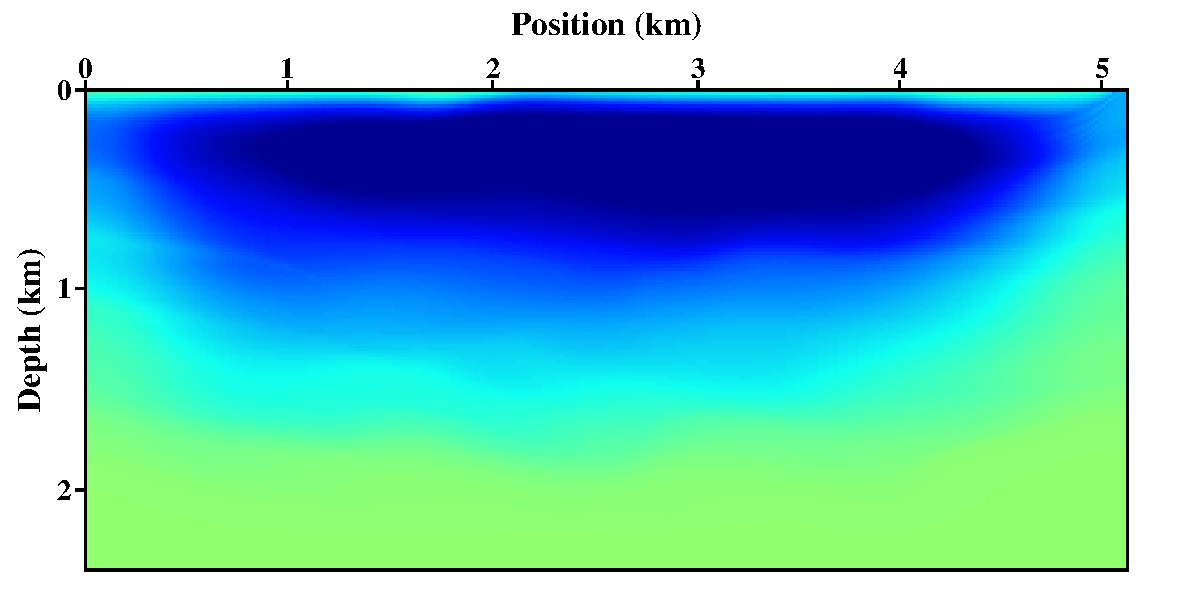
\includegraphics[width=0.48\textwidth]{Figure/chapter03/sigbee2/LSF_Gra_vp.pdf}}
   \subfloat[]{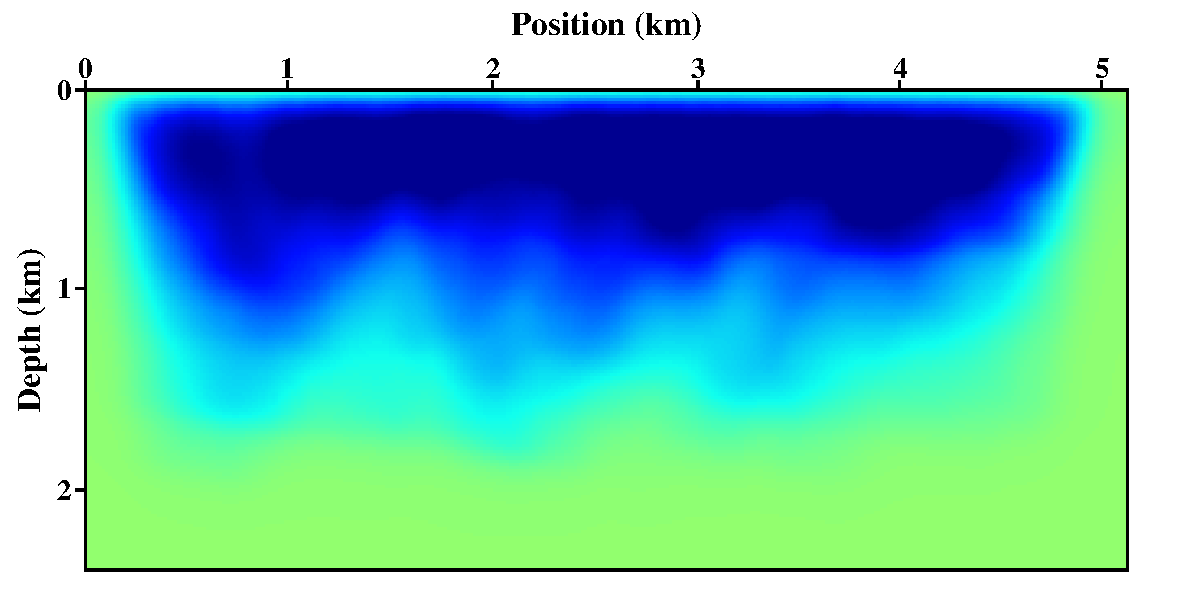
\includegraphics[width=0.48\textwidth]{Figure/chapter03/sigbee2/NoLSF_Gra_vp.pdf}}\\
   \subfloat[]{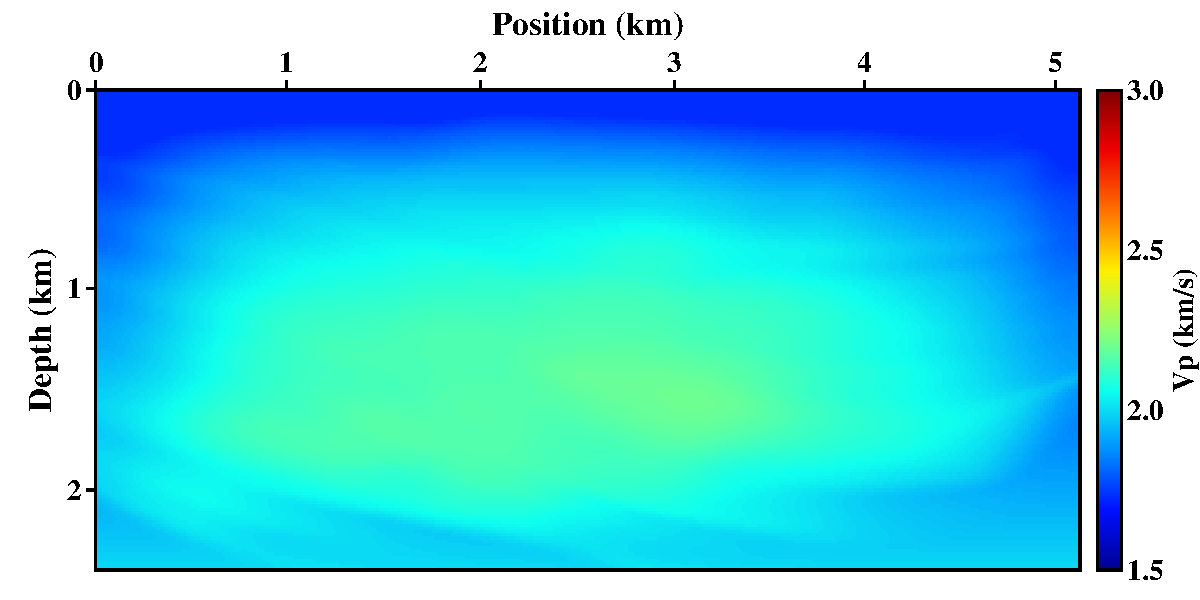
\includegraphics[width=0.48\textwidth]{Figure/chapter03/sigbee2/Fig/newinit3vp.pdf}}
   \subfloat[]{\includegraphics[width=0.48\textwidth]{Figure/chapter03/sigbee2/NoLSF_vp.pdf}}\\
   \caption{局部倾角滤波约束效果展示。(a)和(c)分别为倾角滤波约束下的首次迭代$V_p$梯度与最终反演结果,
   (b)和(d)分别为不加约束时首次迭代的$V_p$梯度与最终反演结果}
   \label{fig:LSF_comparison}
\end{figure}


\begin{figure}[!htb]
   \centering
   \subfloat[]{\includegraphics[width=0.48\textwidth]{Figure/chapter03/sigbee2/Fig/newinit3vp.pdf}}
   \subfloat[]{\includegraphics[width=0.48\textwidth]{Figure/chapter03/sigbee2/Fig/newinit3vs.pdf}}\\
   \subfloat[]{\includegraphics[width=0.48\textwidth]{Figure/chapter03/sigbee2/Fig/nodevp.pdf}}
   \subfloat[]{\includegraphics[width=0.48\textwidth]{Figure/chapter03/sigbee2/Fig/nodevs.pdf}}
   \caption{Inverted results of WERTI and EFWI. (a) and (b) are inverted $V_p$ and
       $V_s$ model through two-stage elastic WERTI with the linearly increased models
       as initial models. (c) and (d) are inverted $V_p$ and $V_s$ through EFWI using
   (a) and (b) as starting models.}
   \label{fig:InvertedModel}
\end{figure}
\begin{figure}[!htb]
   \centering
   \subfloat[]{\includegraphics[width=0.48\textwidth]{Figure/chapter03/sigbee2/Fig/1km.pdf}}
   \subfloat[]{\includegraphics[width=0.48\textwidth]{Figure/chapter03/sigbee2/Fig/3km.pdf}}
   \caption{Vertical profiles of elastic WERTI and EFWI results at 1.4km (a) and
       3km (b). The black and blue lines indicate the true and linearly increased
       initial model. The green and yellow lines indicate the WERTI and EFWI results,
       respectively.
   }
   \label{fig:Profiles}
\end{figure}

采用WERTI的反演结果作为初始模型,我们重新进行了
常规EFWI反演。如图\ref{fig:InvertedModel}c和\ref{fig:InvertedModel}d所示,$V_p$和$V_s$模型都得到了很好的重建,除了模型右侧一小部分。原因可能是在
地面观测下,模型右侧的反射波覆盖不够导致WERTI不能准确的恢复该区域速度的长波长分量。图\ref{fig:Profiles}也展示了1.5km和3km处的垂向剖面。从图中可以看出,
弹性WERTI能够提供可靠的包含长波长分量的初始模型,并且以此为始模型的EFWI反演结果也与真实值很好的吻合。
